\typeout{ ====================================================================}
\typeout{ this is file main.tex, created at 21-Nov-2014               }
\typeout{ maintained by Gustavo Rabello dos Anjos                             }
\typeout{ e-mail: gustavo.rabello@gmail.com                                   }
\typeout{ ====================================================================}

\documentclass[a4paper,portuges,12pt]{article}
\usepackage{babel,varioref,floatflt,wrapfig}
\usepackage{amsmath,booktabs}
\usepackage[utf8]{inputenc}
\usepackage[T1]{fontenc}   % Font Encoding T1 - caracteres acentuados.
\usepackage[top=2.5cm,bottom=2.5cm,left=2.5cm,right=2.5cm]{geometry}
\usepackage{graphicx}    % pacote para inclusao de figuras,
\usepackage{subfig}
%\pagestyle{empty}
\usepackage{indentfirst}
\newcommand{\HRule}{\rule{\linewidth}{0.5mm}}

% removing reference name
\usepackage{etoolbox}
\patchcmd{\thebibliography}{\section*{\refname}}{}{}{}

%%%%%%%%%%%%%%%%%%%%%%%%%%%%%  MACROS MATEMATICOS %%%%%%%%%%%%%%%%%%%%%%%%%%%%%
\newcommand{\tr}{{\,\rm tr}\,}
\newcommand{\sen}{{\,\rm sen}\,}
\newcommand{\senh}{{\,\rm senh}\,}
\newcommand{\diverg}{{\,\rm div}\,}
\newcommand{\grad}{\,\mathbf{grad}\,}
\newcommand{\rot}{\,\mathbf{rot}\,}
\newcommand{\uvet}{\mathbf{u}}
\newcommand{\vvet}{\mathbf{v}}
\newcommand{\wvet}{\mathbf{w}}
\newcommand{\cvet}{\mathbf{c}}
\newcommand{\xvet}{\mathbf{x}}
\newcommand{\gvet}{\mathbf{g}}
\newcommand{\fvet}{\mathbf{f}}
\newcommand{\nvet}{\mathbf{n}}
\newcommand{\tvet}{\mathbf{t}}
\newcommand{\Imat}{\mathbf{I}}
\newcommand{\Eo}{\mathrm{Eo}}
\newcommand{\N}{\mathrm{N}}
\newcommand{\Mo}{\mathrm{Mo}}
%%%%%%%%%%%%%%%%%%%%%%%%%%%%%  MACROS MATEMATICOS %%%%%%%%%%%%%%%%%%%%%%%%%%%%%

\begin{document}	
\typeout{ ====================================================================}
\typeout{ this is file title.tex, created at 21-Nov-2014               }
\typeout{ maintained by Gustavo Rabello dos Anjos                             }
\typeout{ e-mail: gustavo.rabello@gmail.com                                   }
\typeout{ ====================================================================}

\begin{titlepage}
\begin{center}

% Upper part of the page. The '~' is needed because \\
% only works if a paragraph has started.

\includegraphics[width=0.2\textwidth]{./figs/uerj.png}~\\[1cm]

\includegraphics[width=0.3\textwidth]{./figs/gesar.png}~\\[1cm]

\textsc{\LARGE Universidade do Estado do Rio de Janeiro}\\[1.5cm]

\textsc{\Large Relatório Final de Atividades -- CAPES}\\[0.5cm]

% Title
\HRule \\[0.4cm]
{ \huge \bfseries Sistema de Simulação Numérica de Escoamentos
Multifásicos\\[0.4cm] }
{ \Large \bfseries Projeto: A067/2013\\[0.4cm] }
\HRule \\[1.0cm]

% Author and supervisor
\noindent
\large
\emph{Bolsista Jovem Talento:}\\
Gustavo R. \textsc{Anjos}\\
\vspace{0.3cm}
\emph{Coordenador:}\\
Norberto \textsc{Mangiavacchi}\\
\vfill

% Bottom of the page
{\large \today}

\end{center}
\end{titlepage}

\typeout{ ****************** End of file title.tex ****************** }



\tableofcontents
\newpage

\section{Identificação}

\noindent Dados do Coordenador: 
\begin{itemize}
	\item \textbf{Nome:} Norberto Mangiavacchi
	\item \textbf{CPF:} 732.841.227-53
	\item \textbf{Escolaridade:} Doutorado
	\item \textbf{Endereço Profissional:} Rua Fonseca Teles, 121 --
	Prédio Anexo, CEP 20940-903 São Cristóvão, RJ - Rio de Janeiro
	\item \textbf{Telefone Profissional:} +55 21 2332-4733
	\item \textbf{Endereço Eletrônico:} {\tt norberto@uerj.br}, 
	                                    {\tt norberto.mangiavacchi@gmail.com}
	\item \textbf{Página Profissional:} {\tt http://www.gesar.uerj.br}
\end{itemize}

\hspace{1cm}

\noindent Dados do Bolsista: 
\begin{itemize}
	\item \textbf{Nome:} Gustavo Rabello dos Anjos
	\item \textbf{CPF:} 042.432.587-08
	\item \textbf{Escolaridade:} Doutorado
	\item \textbf{Endereço Profissional:} Rua Fonseca Teles, 121 --
	Prédio Anexo, CEP 20940-903 São Cristóvão, RJ - Rio de Janeiro
	\item \textbf{Telefone Profissional:} +55 21 2332-4733
	\item \textbf{Endereço Eletrônico:} {\tt gustavo.anjos@uerj.br}
	\item \textbf{Página Profissional:} {\tt http://www.gesar.uerj.br}
	\item \textbf{Página Pessoal:} {\tt http://gustavo.rabello.org}
\end{itemize}

\clearpage

\section{Resumo}

Após 19 meses de projeto CAPES - Bolsa de Atração de Jovens
Talentos, os objetivos e metas previstos para este período foram
realizados com sucesso. Este documento descreve os resultados obtidos
pelo pesquisador bolsista Gustavo Rabello dos Anjos no projeto
intitulado "Sistema de Simulação Numérica de Escoamentos Multifásicos". 
\clearpage

\section{Introdução}

Deseja-se abordar o desenvolvimento e o estudo numérico de dois
problemas atuais como continuidade de projetos de pesquisa e
desenvolvimento realizados na Universidade do Estado do Rio de
Janeiro/GESAR: 

\begin{itemize}
\item Sistema de simulação numérica de produção, estocagem,
transporte e consumo de metano da decomposição de biomassa em
reservatórios de hidrelétricas (Edital FAPERJ 09/2013 – Programa de
apoio às engenharias 2013); 
\item Simulação numérica de estrutura de
não-equilíbrio em sistemas químicos, biológico e ambientais (Edital de
Cooperação Internacional – Chamada Bilateral CNPq 17/2013 – Bélgica).
\end{itemize}

Ambos com suporte técnico-científico do simulador de escoamentos
multifásicos escrito em linguagem orientada a objetos (MATLAB/C++)
utilizando moderna discretização das equações de governo através do
método de elementos finitos. Para execução do projeto proposto,
planeja-se concluir o desenvolvimento do simulador para modelos
tridimensionais e axisimétricos através da incorporação das seguintes
características: paralelização dos núcleos de cálculo intensivo em
\textit{clusters} baseados em processadores de vários núcleos (
\textit{multicore}), extensa validação do modelo numérico através de
validações analíticas e experimentais, este último com colaboração
internacional, e publicação dos resultados em canais de comunicação
internacionais de excelência. Com isso, objetiva-se o aperfeiçoamento
das técnicas computacionais empregadas na instituição de execução do
projeto (UERJ/GESAR), consolidando o Programa de Pós-graduação em
Engenharia Mecânica na UERJ, e a formação de recursos humanos, com
aperfeiçoamento pessoal de nível superior e pós-graduação. Os
indicadores de desempenho que serão utilizados no projeto estão baseados
em publicações produzidas pelo bolsista na UERJ, juntamente com o aluno
envolvido na bolsa de iniciação científica (IC), e submetidos a
avaliações da comunidade científica.

\section{Objetivos}

\begin{itemize}
	\item estudo e desenvolvimento de modelo em três dimensões e axisimétrico
	      para escoamentos multifásicos;
	\item estudo de escoamentos multifásicos com ondas capilares em bolhas
	      submetidas a campo de temperatura variável;
	\item realização de experimentos computacionais e laboratoriais de
		  decomposição de biomassa e produção de gases com sedimentação
		  de material orgânico; de medição da sedimentação/ressuspensão
		  e consumo de produtos;
	\item validação dos modelos desenvolvidos para sistemas existentes com
	      utilização de tecnologia de última geração;
	\item estudo e desenvolvimento de modelos tridimensionais e axisimétricos
		  para simulação numérica de estrutura de não-equilíbrio em
		  sistemas químicos, biológico e ambientais;
	\item incorporação das seguintes características ao simulador numérico:
		  paralelização dos núcleos de cálculo intensivo em
		  \textit{clusters} baseados em processadores de vários núcleos
		  (\textit{multicore}), através do desenvolvimento de novos
		  precondicionadores para a aceleração dos métodos iterativos
		  implantados e validação do modelo proposto através de soluções
		  analíticas e experimentais (com participação de universidades
		  internacionais);
	\item publicação de resultados em canais de comunicação nacionais e
	      internacionais renomados.
\end{itemize}

\section{Metodologia}

Nesta seção, detalharemos a metodologia utilizada no desenvolvimento do
simulador numérico de escoamentos multifásicos. Para tal, subdividiremos
as seções pela temática da metodologia, a saber: Equações de Governo - 3
dimensões, Equações de Governo - Axissimétrico,
Método de Elementos Finitos, Discretização do Termo de Tensão
Superficial e Solução do Sistema Linear.

\subsection{Equações de Governo}

\subsubsection{Modelo em três dimensões}
\label{sec:3-dimension}

O princípio de conservação de massa estabelece que, dado um fluido
qualquer com massa específica $\rho$ que escoa através de um volume de
controle $V$ invariante no tempo, a taxa de acumulação de massa no
interior do volume é igual ao fluxo líquido de massa para fora do
volume, em módulo. Para o problema proposto neste trabalho, onde não há
variação da massa específica do fluido em cada fase, ou seja, a massa
específica é constante em cada fase, a equação de conservação de massa
representada em coordenadas cartesianas para três dimensões é escrita como:

\begin{equation}
	\frac{\partial v_x}{\partial x} +
	\frac{\partial v_y}{\partial y} +
	\frac{\partial v_z}{\partial z}  
	= 
	0
	\label{eq:cm9}
\end{equation}\vspace{0.5cm}

Para obtenção das equações de conservação da quantidade de movimento
linear para fluidos newtonianos realiza-se o mesmo procedimento de
obtenção da equação de conservação de massa. O princípio de conservação
da quantidade de movimento estabelece que, dado um fluido qualquer com
massa escoa específica $\rho$ que escoa através de um volume de controle
V, a taxa de acumulação de quantidade de movimento é igual ao fluxo
líquido de quantidade de movimento para fora do volume mais a resultante
das forças de superfície e de volume. A equação de conservação de
quantidade de movimento linear representada em coordenadas cartesianas é
dada por:

\begin{equation}
	\frac{\partial \vvet}{\partial t} + \vvet \cdot \nabla \vvet
	= 
	- \frac{1}{\rho} \nabla p +
	\nabla \cdot [\nu(\nabla \vvet + \nabla \vvet^T)] + 
	\textbf{g} + 
	\textbf{f}
\label{eq:NS3a}
\end{equation}\vspace{0.5cm}

O princípio do transporte de energia estabelece que, dado um
fluido qualquer com massa específica $\rho$ que escoa através de um
volume de controle V, a taxa de acumulação da quantidade de energia
que entra no volume por unidade de tempo é igual ao fluxo
líquido de massa para fora do volume, na ausência de termos relacionados
ao trabalho e a dissipação toma a forma final representada em
coordenadas cartesianas como:

\begin{equation}
	\frac{\partial T}{\partial t} + \vvet \cdot \nabla T
	=  
	\nabla \cdot (k \nabla T)
\label{eq:quimica2}
\end{equation}\vspace{0.5cm}

É conveniente adimensionalizarmos as equações de conservação acima
citadas através de parâmetros conhecidos, como o diâmetro da bolha,
diâmetro do canal de escoamento dos fluidos e velocidade de escoamento.
Com isso analisamos os escoamentos através de números adimensionais que
podemos comparar com diversos problemas encontrados na literatura. As
equações de conservação em sua forma final adimensionalizada são
descritas como:

\begin{equation}
	\frac{\partial \vvet}{\partial t} + \vvet \cdot \nabla \vvet
	=
	-\frac{1}{\rho} \nabla p + \frac{1}{Re} \nabla \cdot
	[\nu ( \nabla \vvet + \nabla \vvet^T)]+
	\frac{1}{Fr^2} \mathbf{g} + 
	\frac{1}{We} \mathbf{f}
	\label{eq:final1}
\end{equation}
\begin{equation}
	\diverg \cdot \vvet = 0
	\label{eq:final2} 
\end{equation}	
\begin{equation}
	\frac{\partial T}{\partial t} + \vvet \cdot \nabla T
	=
	\frac{1}{RePr} \nabla \cdot (k \nabla T)
	\label{eq:final3}
\end{equation}\vspace{0.5cm}

\noindent onde $Fr$ representa o número de \textit{Froud}, $Re$
representa o número de \textit{Reynolds}, $We$ representa o número de
\textit{Weber} e todas as outras variáveis estão eu sua forma
adimensional.

Para solução do problema de escoamentos multifásicos, procuramos então
encontrar a solução dos campos de velocidade $\vvet$, pressão $p$ e
temperatura $T$ enunciados nos três princípios de conservação descritos
acima. Como a solução analítica destas equações são restritas a
pouquíssimos casos práticos, onde muitas simplificações são realizadas,
utilizamos uma metodologia numérica de aproximação de solução para
encontramos os valores dos campos $\vvet$, $p$ e $T$ em geometrias
complexas que são pertinentes ao projeto proposto. 

O termo que representa a força de tensão superficial
$(\mathbf{f}(f_r,f_z)$ é calculado através do método de modelagem da
força de tensão superficial contínua sugerido por \cite{brackbill1992}:

\begin{equation}
	\mathbf{f} = \sigma \kappa \nvet \delta 
\label{eq:brackbill}
\end{equation}\vspace{0.5cm}

\noindent onde $\sigma$ é o valor do coeficiente de tensão superficial,
$\kappa$ representa a curvatura, $\nvet$ o vetor normal à superfície que
separa os fluidos e $\delta$ representa uma função de identificação da
posição da interface.

\subsubsection{Modelo axissimétrico}
\label{sec:axi}

Para o caso de um modelo bidimensional axissimétrico, faz-se a hipótese
de que o escoamento é simétrico em torno do eixo longitudinal $z$ em um
sistema de coordenadas cilíndricas $(r,\theta,z)$. Matematicamente, esta
hipótese é escrita como $d/d\theta=0$ onde $\theta$. Com esta hipótese
de simetria e a utilização do sistema de coordenadas cilíndricas, as
equações de conservação de quantidade de movimento linear para as duas
componentes $r$ e $z$ tomam a forma de:

\begin{equation}
	\frac{\partial v_r}{\partial t} + \vvet \cdot \nabla v_r
	= 
	- \frac{1}{\rho} \frac{\partial p}{\partial r} +
	\nabla \cdot [\nu(\nabla v_r + \nabla v_r^T - \frac{v_r}{r^2})] 
	+ 
	f_r
\label{eq:NSAxi1}
\end{equation}

\begin{equation}
	\frac{\partial v_z}{\partial t} + \vvet \cdot \nabla v_z
	= 
	- \frac{1}{\rho} \frac{\partial p}{\partial z} +
	\nabla \cdot [\nu(\nabla v_z + \nabla v_z^T)] + 
	g_z 
	+ 
	f_z
\label{eq:NSAxi}
\end{equation}\vspace{0.5cm}

Para a inclusão da hipótese de simetria na equação de conservação de
massa, é necessário incluir um termo da componente de velocidade $v_r$
dividido pelo raio $r$ e que para um sistema bifásico toma a forma de:

\begin{equation}
	\frac{\partial v_r}{\partial r}
	+
	\frac{v_r}{r}
	+
	\frac{\partial v_z}{\partial z}  
	= 
	0
	\label{eq:cm9-axi}
\end{equation}\vspace{0.5cm}

O operador laplaciano $\nabla^2$ é representado por:

\begin{equation}
	\nabla^2 
	=
	\frac{\partial^2}{\partial r^2}
	+
	\frac{1}{r}
	\frac{\partial}{\partial r}
	+
	\frac{\partial^2}{\partial z^2}
\label{eq:laplacianAxi}
\end{equation}\vspace{0.5cm}

O termo que representa a força de tensão superficial
$(\mathbf{f}(f_r,f_z)$ é calculado através do mesmo método apresentado
anteriormente para o modelo em três dimensões, entretanto, para o
correto cálculo da tensão superficial em um modelo axissimétrico, se faz
necessária a inclusão da curvatura na direção de rotação do eixo de
simetria $r$, ou seja, a curvatura referente à direção de $\theta$:

\begin{equation}
	\kappa = \kappa_{2D} + \frac{sen(\phi)}{r}
\label{eq:curvAxi}
\end{equation}\vspace{0.5cm}

\noindent onde $r$ é a distância do elemento infinitesimal do campo ao
eixo de simetria $z$ através da reta paralela ao vetor normal da
interface entre os dois fluidos. Esquematicamente, este modelo está
representado pela Fig~(\ref{fig:axisymmetric})

 \begin{figure}[h!]
 	\begin{center}
 		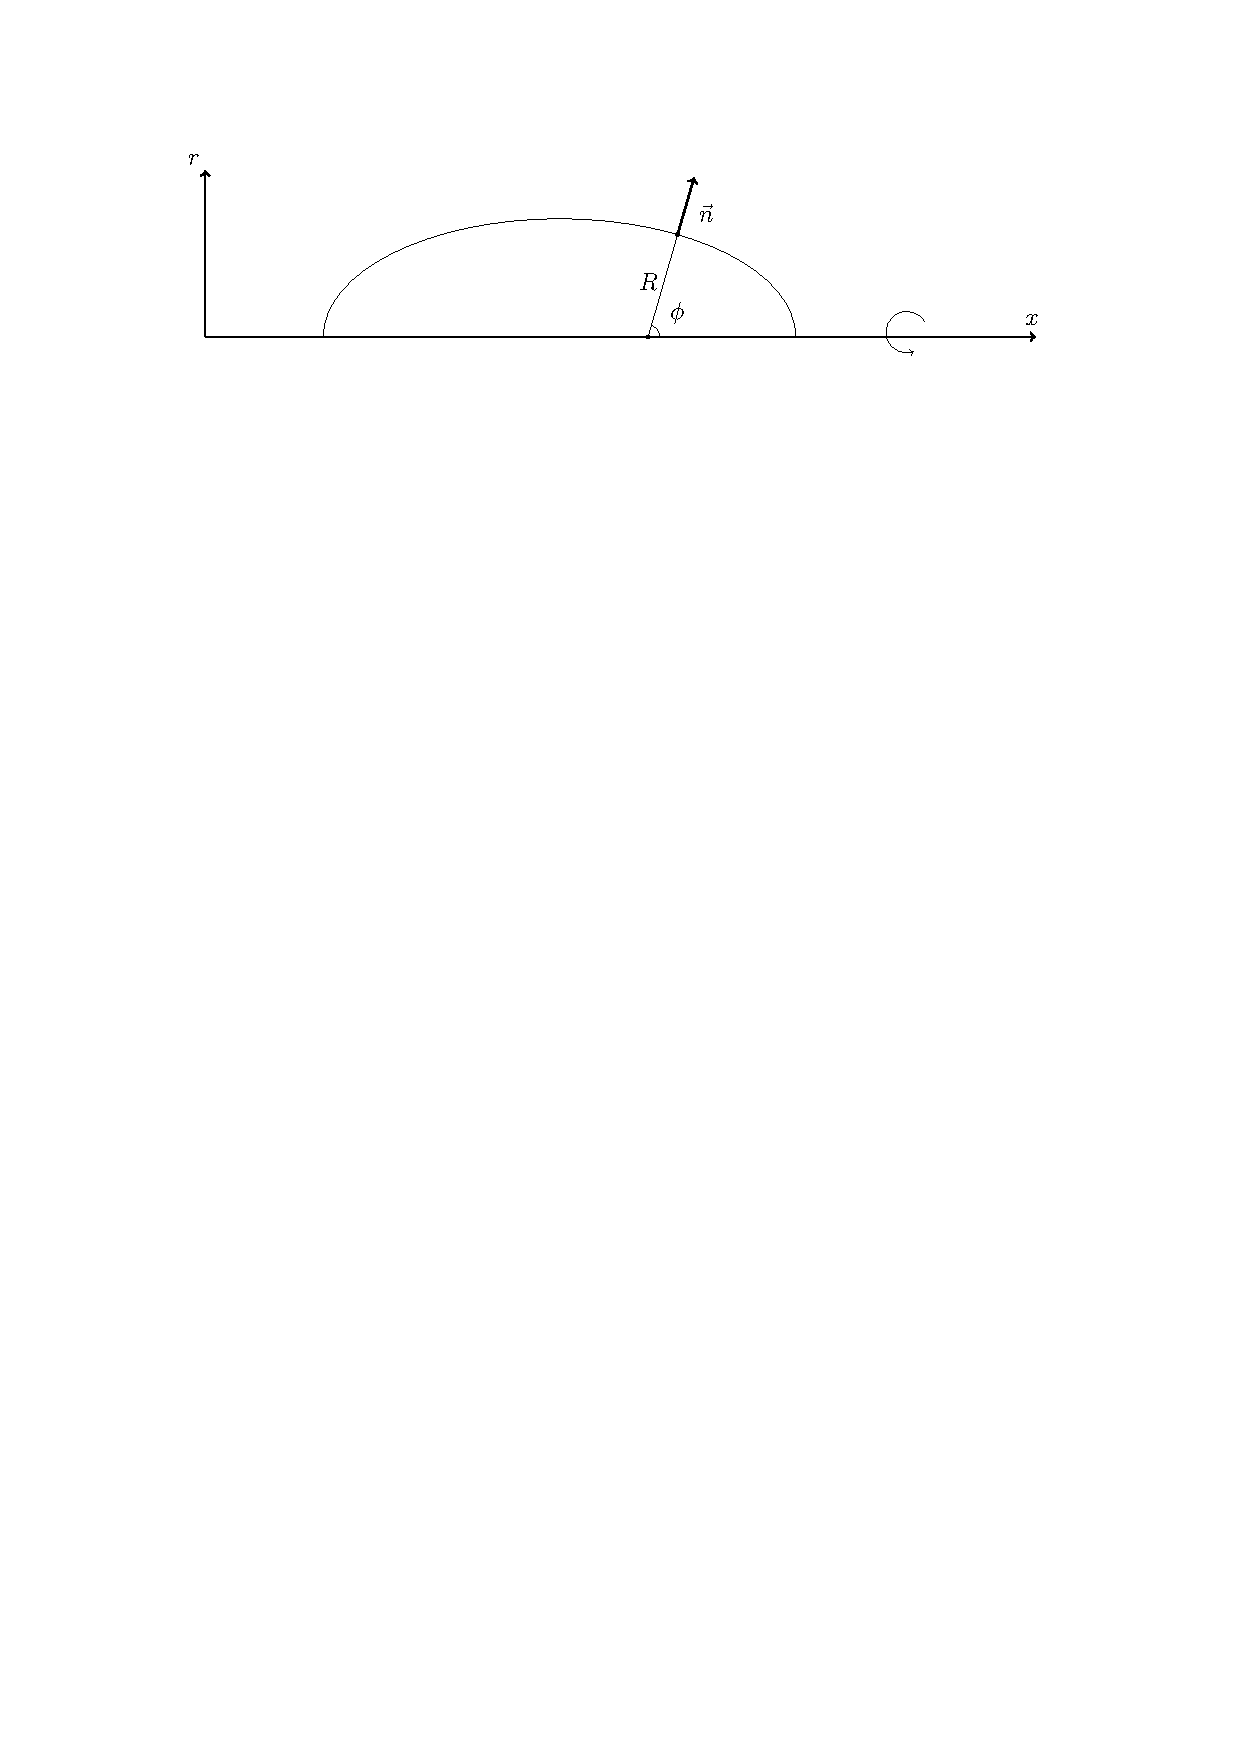
\includegraphics[angle=0, scale=0.5]{figs/axisymmetric.pdf}
 	\end{center}
	\caption{Representação esquemática de cálculo da curvatura para o
	caso das equações de governo em modelo axissimétricas, onde $r$ é a
	distância do elemento infinitesimal do campo ao eixo de simetria $z$
	através da reta paralela ao vetor normal da interface entre os dois
	fluidos. }
 	\label{fig:axisymmetric} 
 \end{figure}

\subsubsection{Modelo de estruturas de não-equilíbrio em sistemas
químicos}
\label{sec:chem}

Modelo de estruturas de não-equilíbrio refere-se a instabilidades
hidrodinâmicas de interfaces de separação de fluidos em meios porosos.
Estas instabilidades estão fortemente ligadas a variações de viscosidade e
densidade em camadas distintas de uma fase líquida contendo
concentrações de soluto que afetam diretamente as propriedades do
líquido. Este fenômeno ocorre em uma grande variedade de aplicações
industriais, incluindo técnicas de sequestro de $CO_2$, hidrologia,
filtragem, cromatografia de líquidos e tantas outras. 

No modelo proposto, considera-se o problema de geração de estruturas
através de escoamento caracterizado por empuxo, gerado em meios porosos
devido à dissolução de uma camada de líquido inicialmente posicionada
sobre outra camada de líquido de densidade menor. Matematicamente, este
modelo é governado pela lei de Darcy e a aproximação de Boussinesq para
devida consideração dos efeitos de empuxo provocados pela diferença de
densidade. As equações que descrevem a dinâmica e evolução do escoamento
são apresentadas em uma formulação corrente-vorticidade com acoplamento
da equação de concentração:

\begin{equation}
	\nabla^2 \psi = -\omega_z
\label{eq:chem1}
\end{equation}

\begin{equation}
	\omega_z = R \frac{\partial c}{\partial x}
\label{eq:chem2}
\end{equation}

\begin{equation}
	\frac{D c}{D t} = D \nabla^2 c
\label{eq:chem3}
\end{equation}\vspace{0.5cm}

\noindent onde $\psi$ representa a função corrente, $\omega_z$ a função
vorticidade, $c$ a concentração da solução, $R$ um parâmetro do
problema, $D$ o coeficiente de difusão de massa e $t$ representa o
tempo.

\subsection{Método de Elementos Finitos}

Nos anos 50, o método de elementos finitos teve grande utilização na
mecânica de sólidos.  Apenas a partir da década de 70, após a
consolidação do método de Galerkin para equações de difusão,
pesquisadores começaram a investir no campo da dinâmica dos fluidos,
pode-se citar \cite{zienkiewicz1965}, \cite{oden1972}, \cite{oden1998},
\cite{chung1978}, \cite{hughes1982}, \cite{pironneau1989} e tantos
outros.  Em seguida, vários autores contribuíram para o desenvolvimento
de metodologias específicas como métodos de Petrov-Galerkin
generalizados \cite{heinrich1977}, \cite{hughes1986},
\cite{johnson1987}, métodos adaptativos \cite{oden1989}, métodos de
Taylor-Galerkin \cite{donea1984}, \cite{lohner1985}, método de Galerkin
descontínuo \cite{oden1998} etc.

O começo relativamente tardio no campo da Física de fluidos se deve,
principalmente, à presença do termo convectivo e ao forte acoplamento
entre velocidade e pressão, presentes nas equações de conservação. O
termo convectivo apresenta produto de incógnitas, caracterizando a
não-linearidade do problema e gerando operadores não simétricos, de
difícil solução.  Com o aumento do número de \emph{Reynolds}, o termo
convectivo exerce maior influência no escoamento, aumentando ainda mais
a dificuldade de solução das equações.

Outra fonte de dificuldade numérica é a condição de incompressibilidade,
que consiste em manter o campo de velocidade com divergência zero.
Então, a pressão deve ser considerada uma variável não relacionada a
qualquer equação constitutiva.  Sua presença nas equações de conservação
de quantidade de movimento tem o propósito de introduzir um grau de
liberdade a mais necessário para satisfazer a condição de divergência
zero do campo de velocidades.  Isto é, a pressão atua como um
multiplicador de Lagrange na condição de incompressibilidade resultando
em um acoplamento entre velocidade e pressão desconhecidas.

\subsection{Discretização do Termo de Tensão Superficial}

Em códigos do tipo \textit{front-tracking} a construção da interface é feita
através de um conjunto de objetos geométricos, como triângulos,
segmentos de reta e nós, que são movidos na forma lagrangiana, onde a
malha tridimensional é fixa no espaço. Uma função adicional é necessária
para comunicação entre as malhas, uma vez que não há nenhuma
interconectividade implícita. Esta abordagem mantém a interface entre as
fases com espessura zero, no qual uma representação precisa é obtida.
Apesar de sua ótima definição geométrica , as propriedades do fluido
perto da interface exigem tratamento numérico para evitar instabilidades
indesejáveis. Como consequência, estas propriedades são suavizados ao
longo da zona de transição e a espessura nula já não pode ser mais
garantida.

Ao contrário de códigos do tipo \textit{front-tracking}, a malha da interface
faz parte da malha tridimensional. Com isso não há necessidade do uso de
uma equação de transporte adicional ao modelo proposto. A malha
3-dimensional compreende um conjunto de elementos tetraédricos
distribuídos sobre o domínio e a interface é encontrado por uma função
escalar, ou seja, uma função do tipo \textit{Heaviside}, que define os nós que
pertencem a cada uma das fases mais a interface em si. Para obter uma
representação zero espessura, os nós da interface devem ser ligado de
forma consistente para que sua discretização possa ser representado por
um conjunto de triângulos interligado. Em outras palavras, cada
triângulo é uma face de dois elementos tetraédricos adjacentes. A
Fig~(\ref{fig:inter}a) mostra um diagrama esquemático da
representação da interface entre as duas fases discretas. A mesma face
do triângulo é compartilhada por dois tetraedros adjacentes, por
conseguinte, a interface de espessura zero é obtida com sucesso.

\begin{figure}[ht!]
		\subfloat[]{
		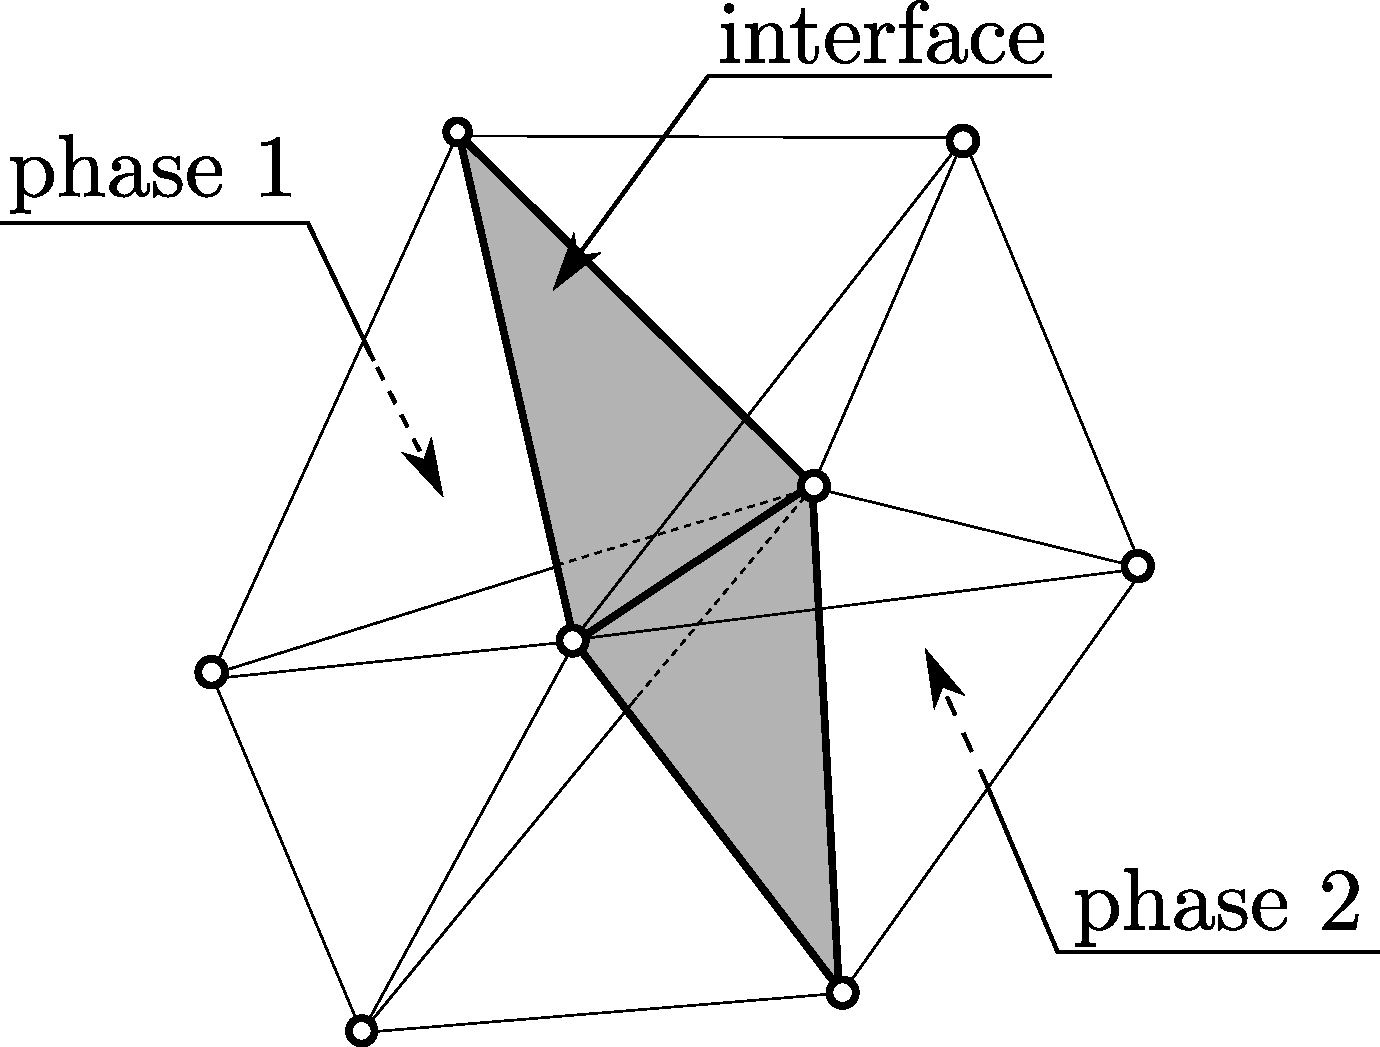
\includegraphics[scale=0.3]{figs/interface.pdf}}
		\subfloat[]{
		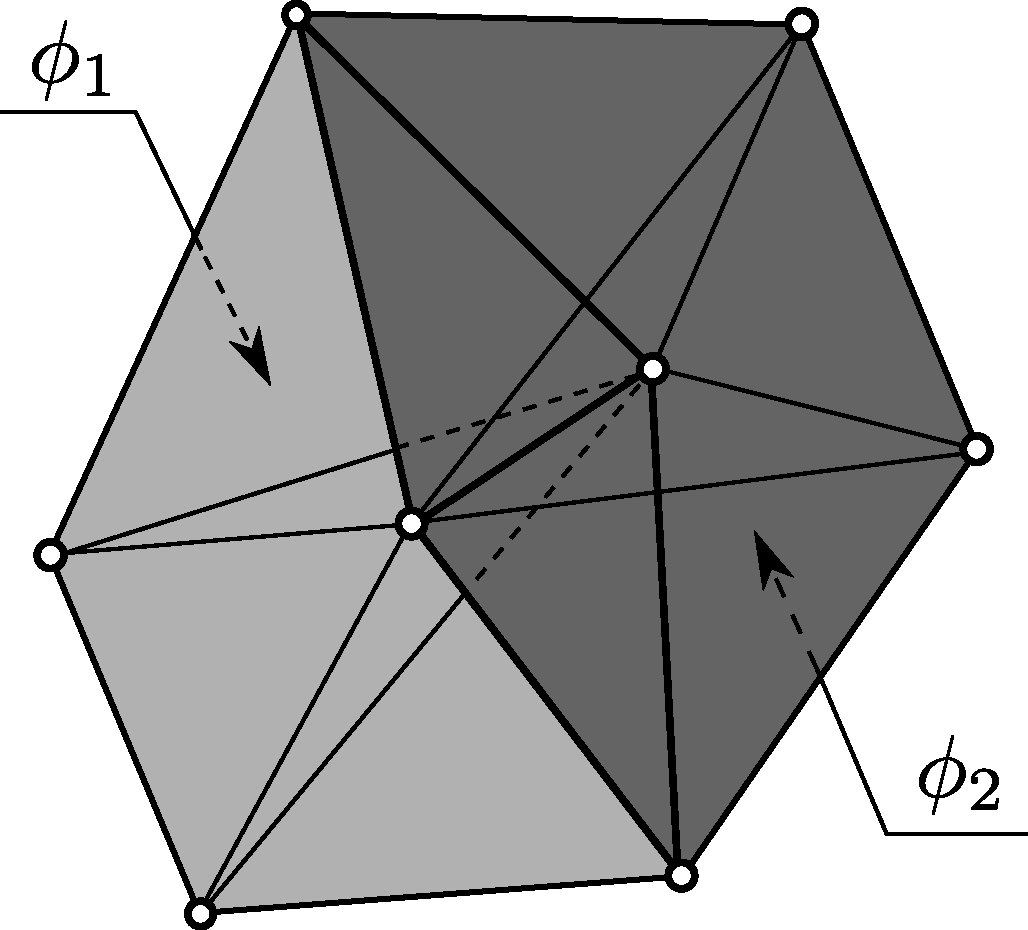
\includegraphics[scale=0.3]{figs/property.pdf}}
	\caption{Representação geométrica da interface entre as fases. (a) A
	interface (em cinza) é representada por um conjunto de triângulos,
	segmentos de retas e nós que fazem parte da malha de tetraedros. (b)
	(b) A propriedade do fluido $\phi$, tal como densidade ou
	viscosidade, é definida precisamente na fase $1$ e na fase $2$ com 
	espessura zero na zona de transição das fases.}
	\label{fig:inter} 
\end{figure}

Pontos negativos e positivos são encontrados nesta abordagem numérica,
mas uma característica é especialmente interessante devido à definição
das propriedades do fluido na área de transição. Do ponto de vista
macroscópico, o significado físico de uma interface é a região que
divide acentuadamente o volume ocupada por cada fase. Assim, é desejável
que uma tal uma espessura de interface deve ser mantida tão fina quanto
possível. A descrição lagrangiana garante a parte geométrica, mas,
devido à mudança brusca nas propriedades de uma fase para outra,
instabilidades numéricas podem aparecer e deteriorar a precisão da
solução. Tal problema é devido à localização da interface entre dois
elementos computacionais. Isso pode ser contornado com a formulação ALE
aliada ao método de Elementos Finitos, em que a interface não fica
localizada entre elementos de malha mas compartilha as faces de dois
elementos computacionais adjacentes e, assim, as propriedades do fluido
permanecem constante em cada elemento de malha. A transição brusca de
propriedades é, portanto, obtida com sucesso e não requer a utilização
de qualquer funções de suavização, consequentemente, garantindo precisão
no equilíbrio de forças próximas à interface.

Figura~(\ref{fig:inter}b) mostra a zona de transição entre as duas fases
coloridas por cinza claro e escuro, que foi propositadamente desenhadas
para destacar a metodologia proposta deste trabalho. Como pode ser
visto, a propriedade $\phi_1$ preenche os elementos da fase 1 e a
propriedade $\phi_2$ preenche exatamente os elementos de fase 2. Mesmo
para uma razão de propriedade alta $\phi_1 / \phi_2 =$ 1000, a
metodologia proposta aqui não apresenta oscilações espúrias nos campos
de pressão e velocidade. Devido à formulação de elementos finitos, cada
propriedade $\phi$ é atribuída em cada elemento tetraédrico, assim, uma
transição brusca de propriedades é obtida. Este procedimento de
suavização é necessário para evitar instabilidades numéricas perto da
interface.

Apesar da definição precisa da interface e das transição das
propriedades dos fluidos, mudanças topológicas não são naturalmente
inerentes nesta metodologia, requisitando então um esforço de
implementação na modelagem de coalescência e quebra de interface de
bolhas e gotas. Entretanto, com o uso adequando de modelos geométricos
pode-se modelar a separação e colapso de duas interfaces distintas. Por
exemplo, quando a espessura do filme de líquido que separa duas bolhas
diminui até um determinado valor, as superfícies das bolhas são
conectadas e obtém-se a coalescência das bolhas. Apesar das mudanças
topológicas ocorrerem, os aspectos físicos do problema não são
solucionados. É fato que o problema físico de coalescência de bolhas e
quebra de interface ainda é tema de pesquisas atuais.

Uma formulação baseada em elementos finitos pode ser encontrada para a
força de tensão superficial considerando o seguinte esquema: 

\begin{equation}
	\frac{1}{We}\mathbf{M} \fvet 
	= 
	\frac{1}{We} \mathbf{\Sigma} \mathbf{G} H_{\lambda}
	\label{eq:surfDiscrete}
\end{equation}\vspace{0.5cm}

Na equação acima, $\mathbf{\Sigma}$ representa uma matriz diagonal com
elementos $\sigma \kappa_1, \sigma \kappa_2, \sigma \kappa_3,$ $\cdots,
\sigma \kappa_{NV}$, onde $NV$ é o número total de nós da malha
relativos ao campo de pressão. A matriz $\mathbf{G}$ representa a forma
discreta do operador gradiente $\nabla$ e $H_{\lambda}$ é o função
discreta \textit{Heaviside}. Equação~(\ref{eq:surfDiscrete}) pode ser
substituída na forma discreta da equação de conservação de quantidade de
movimento e o termo de tensão superficial pode então ser calculado. 

\section{Atividades Desenvolvidas pelo Bolsista JVT e Bolsista IC}

Pelo beneficiário da bolsa de Atração de Jovens Talentos: Gustavo Rabello
dos Anjos
\begin{itemize}
	\item estudo e desenvolvimento de modelo em três dimensões e axisimétrico
	para escoamentos multifásicos;
	\item estudo de escoamentos multifásicos com ondas capilares em bolhas
	submetidas a campo de temperatura variável;
	\item realização de experimentos computacionais e laboratoriais de
	decomposição de biomassa e produção de gases com sedimentação de
	material orgânico; de medição da sedimentação/ressuspensão e consumo de
	produtos;
	\item validação dos modelos desenvolvidos para sistemas existentes com
	utilização de tecnologia de última geração;
	\item estudo e desenvolvimento de modelos tridimensionais e axisimétricos
	para simulação numérica de estrutura de não-equilíbrio em sistemas
	químicos, biológico e ambientais;
	\item incorporação das seguintes características ao simulador numérico:
	paralelização dos núcleos de cálculo intensivo em \textit{clusters}
	baseados em processadores de vários núcleos (\textit{multicore}),
	através do desenvolvimento de novos precondicionadores para a
	aceleração dos métodos iterativos implantados e validação do modelo
	proposto através de soluções analíticas e experimentais (com
	participação de universidades internacionais);
	\item publicação de resultados em canais de comunicação nacionais e
	internacionais renomados.
\end{itemize}

Pelos beneficiários da bolsa de Iniciação Científica: Vinícius Augusto
Cinquini Mascarenhas e Paulo Roberto Berti Leite Filho

\begin{itemize}
	\item Revisão bibliográfica pertinente ao projeto;
	\item familiarização com as técnicas desenvolvidas e implementadas no
	código numérico;
	\item execução de testes no código numérico;
	\item aumento da qualificação profissional do aluno de IC através de
	desenvolvimento e pesquisa.
\end{itemize}

\section{Resultados Obtidos}

Nesta seção, detalharemos os resultados obtidos através do
desenvolvimento do simulador numérico de escoamentos multifásicos. Para
tal, subdividiremos as seções pela temática da metodologia, a saber: 
 
\begin{itemize}
	\item Modelo em três dimensões: resultados obtidos através da
	discretização das equações de conservação de massa, quantidade de
	movimento e energia (temperatura) em três dimensões cartesianas;
	\item Modelo axissimétrico: resultados obtidos através da
	discretização das equações de conservação de massa e quantidade de
	movimento para problemas com simetria axial;
	\item Modelo de estruturas de não-equilíbrio em sistemas químicos:
	resultados obtidos através da discretização da equação de Darcy em
	uma formulação corrente-vorticidade e conservação de energia
	(concentração).
\end{itemize}

\subsection{Modelo em três dimensões}

Nesta seção buscamos apresentar algumas validações e resultados obtidos
com o desenvolvimento do código de elementos finitos tridimensionais
para simulação de escoamentos multifásicos. As
Figs.~(\ref{fig:pressure3d}, \ref{fig:oscillating} e
\ref{fig:sessileShape})
representam validações através de comparação com resultados analíticos.
A Fig.~(\ref{fig:sucrose}) é resultado de simulação de bolha de ar
imersa em uma solução de sacarose confinada em um canal vertical, movida
devido a força gravitacional (empuxo). Enquanto que na
Fig.~(\ref{fig:sucroseVel}) mostra-se o perfil de velocidade do centro
de massa da bolha em função do tempo para o mesmo caso. Na
Fig.~(\ref{fig:sin}), mostra-se uma simulação numérica de escoamento
multifásico de uma bolha de ar imersa em uma solução de glicerol em um
canal com formato senoidal. Nele é possível notal que a bolha é
comprimida e alongada devido a passagem em partes mais estreitas do
canal seguida de passagens com expansão. Neste projeto também foram
realizadas simulações utilizando o recém desenvolvido simulador
com modelo axissimétrico para cálculos de bolhas em ascensão e bolhas em
microcanais. Para o problema de estruturas de
não-equilíbrio em sistemas químicos, biológico e ambientais, foram
realizados diversos testes, onde os dois mais importantes estão
ilustrados nas próximas seções, no qual perfis de concentração médios
para diversos passos de tempo são ilustrado e comparados a soluções
analíticas. 

\subsubsection{Gota estáticas}

Neste teste buscamos analisar o acoplamento entre pressão e tensão
superficial e a consequente geração de escoamentos espúrios devido à
discretização numérica da equação de conservação. Nele, inicializamos
uma gota esférica e imersa em outro fluido na ausência de qualquer força
externa e campo de velocidade. Matematicamente a equação de quantidade
de movimento Eq.~(\ref{eq:NS3a}) se reduz a:

\begin{equation}
	\nabla p = \fvet
\end{equation}

Esta equação mostra que a força de tensão superficial está em equilíbrio
com o gradiente de pressões. Entretanto, devido à discretização
numérica, correntes espúrias de velocidade podem aparecer como resultado
devido às várias aproximações realizadas no decorrer do código numérico.
Tal efeito não é desejável e objetiva-se minimizá-lo, de tal forma que
os erros provenientes à discretização dos termos não afete o resultado
em uma simulação mais rigorosa. 

Na Fig.~(\ref{fig:pressure3d}) o teste de gota estática é realizado com
sucesso, mostrando que a pressão é exercida na bolha é proporcional
à tensão superficial de uma gota com raio $R=0.5$ e $Eo=0.2$, resultando
em uma diferença de pressão $\Delta P = 20$.

 \begin{figure}[h]
 	\begin{center}
 		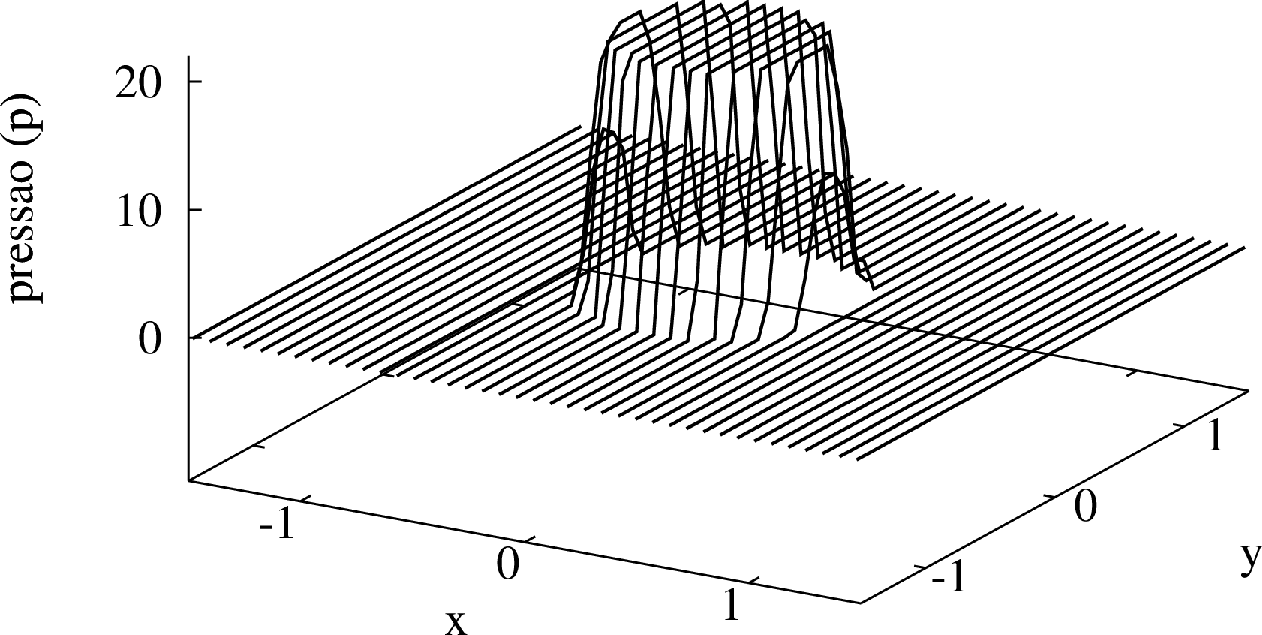
\includegraphics[angle=0, scale=0.5]{figs/pressure3d.pdf}
 	\end{center}
 	\caption{Pressão capilar de uma gota esférica imersa em outra fluido. 
	O salto de pressão pode ser visto na localização da interface que
	separa os fluidos.}
 	\label{fig:pressure3d} 
 \end{figure}

\subsubsection{Gota oscilante}

A evolução de uma gota inicialmente perturbada diametralmente é
apresentada neste caso teste. Este, é parte de um conjunto de testes
essenciais para validação de problemas envolvendo dinâmica de
escoamentos com presença de tensão superficial. A simulação consiste em
inicializar uma gota elipsoidal e simétrica axialmente na ausência de
campos gravitacionais. Assumindo que os efeitos de viscosidade são
mínimos, espera-se que a gota perturbada oscile diametralmente devido à
variação de pressão e tensão superficial. Esta oscilação é caracterizada
por uma frequência analítica, descrita por:

\begin{equation}
	w^2 = \frac{24\sigma}{(3\rho_{in}+2\rho_{out})R^3 }
\label{eq:frequency}
\end{equation}

\noindent e um decaimento de amplitude dado por:

\begin{equation}
	a(t) = a_0 e^{-t/\tau}
\label{eq:amplitude}
\end{equation}

\noindent onde $\rho_{in}$ representa a densidade da gota, $\rho_{out}$
representa a densidade do fluido externo à gota e $R$ é o raio da gota
não perturbado. Na equação de amplitude, $a_0$ é o valor inicial da
amplitude da gota que deve ser pequeno o bastante para evitar o
crescimento de modos não-lineares. O tempo é dado por $t$ e $\tau=R/5\nu$
onde $R$ é o raio da gota não perturbado e $\nu$ é a viscosidade
cinemática. Para esta simulação, $a_0$ foi ajustado para o valor de
$0.1R$, garantindo a linearização do processo de perturbação. 

A Fig.~(\ref{fig:oscillating}) mostra a solução numérica para a
posição axial da interface para dois diferentes refinamentos de malha,
chamados de "coarse" (grosseiro) e "refined" (refinado). A comparação é
então feita através da curva analítica para posição de um ponto na
interface dado por:

\begin{equation}
	y(t) = y_0 + a_0 e^{-t/\tau} cos(wt).
\label{eq:oscillating}
\end{equation}

\noindent onde $y_0$ corresponde a posição inicial da interface
perturbada, $t$ representa o tempo e $w$ a frequência de oscilação. A
amplitude inicial é ajustada por $a_0$. Como esperado, a curva para a
malha refinada apresenta melhor concordância com a curva analítica dada
pela Eq.~(\ref{eq:oscillating}).

 \begin{figure}[h!]
 	\begin{center}
 		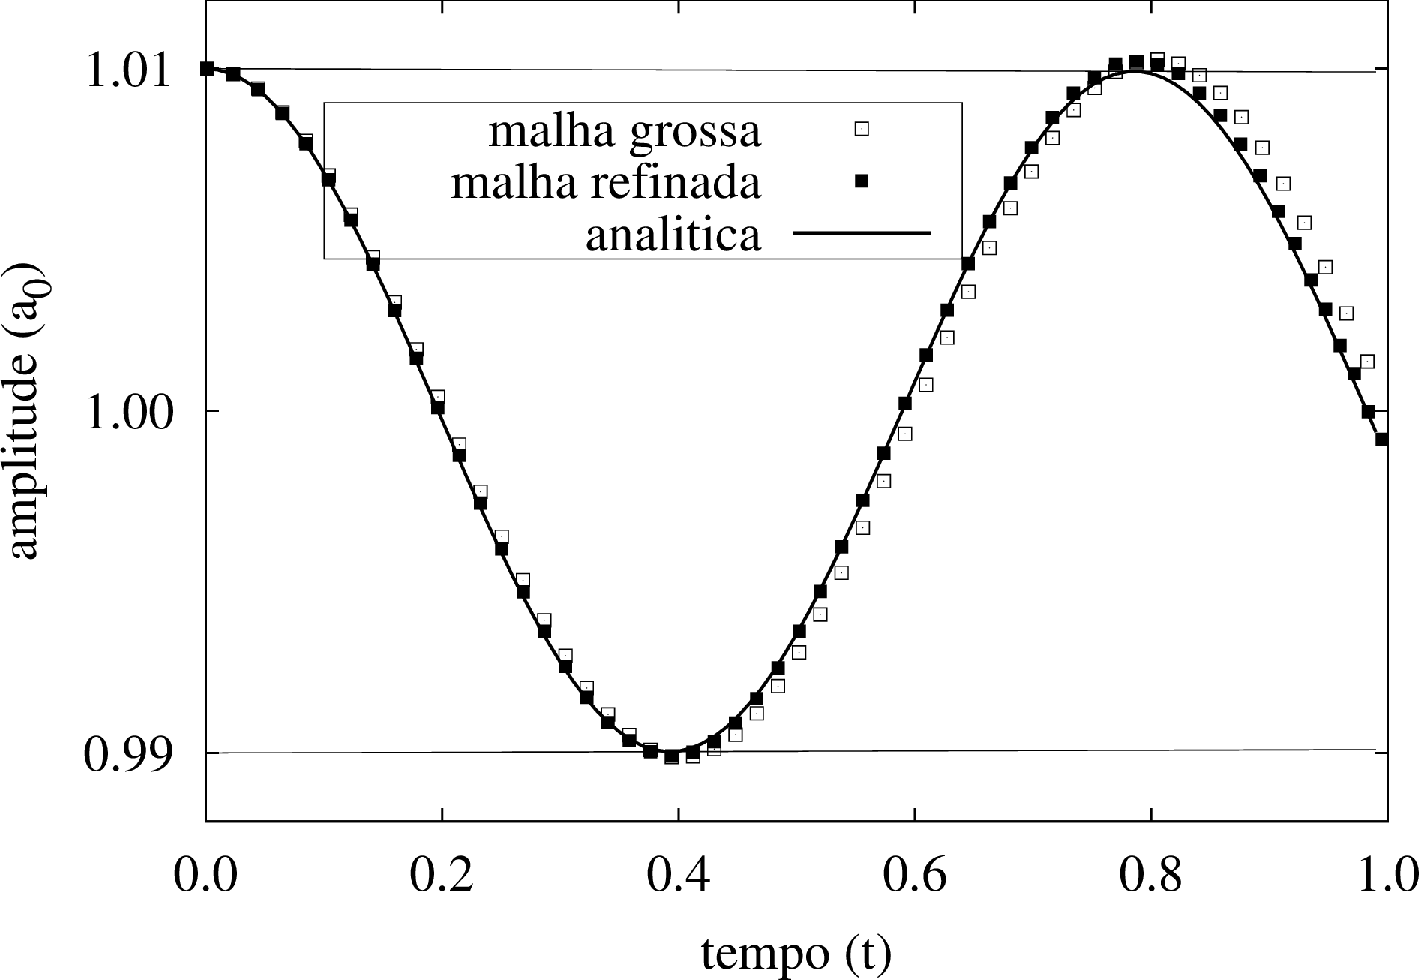
\includegraphics[angle=0, scale=0.5]{figs/oscillating.pdf}
 	\end{center}
	\caption{Amplitude de oscilação de uma gota. Comparação entre a
	solução numérica através do método de elementos finitos e a solução
	analítica para dois níveis de refinamento de malha. O período
	analítico é $0.785$ e a taxa de decaimento é mostrada pelas linhas
	abaixo e acima da curva de oscilação. O período encontrado para a
	malha grossa foi de $0.820$ enquanto que para a malha refinada foi
	de $0.783$.}
 	\label{fig:oscillating} 
 \end{figure}

\subsubsection{Gota apoiada}

Neste teste foi validada a implementação do termo de tensão superficial
$\fvet$ e seu acoplamento com o termo de pressão e gravidade. Uma gota
esférica de raio $R=0.5$ é inicialmente colocada próxima a uma
superfície rígida. Devido à diferença de densidades, a gota se movimenta
verticalmente para baixo até tocar na parede. Neste teste, estamos
interessados em comparar a forma da gota instantes antes da mesma tocar
a superfície rígida. Esta forma pode ser comparada através da
clássica solução de Young-Laplace para gotas que se escreve como se
segue:

\begin{equation}
	\big( \frac{1}{R_1}+\frac{1}{R_2} \big)\frac{1}{Eo}
	=
	\Delta p_g
	=
	\Delta \rho g (z-z_0)
	\label{eq:young-laplace}
\end{equation}

\noindent onde $R_1$ e $R_2$ são os dois principais raios com simetria
axial da bolha, $\sigma$ representa o coeficiente de tensão superficial,
e$\Delta p_g$ a diferença de pressão hidro-estática através da
interface, onde $\Delta \rho = \rho_{in}-\rho_{out}$. 

A forma da bolha antes de tocar na superfície rígida é comparada com sua
solução analítica dada pela Eq.~(\ref{eq:young-laplace}) e mostrada na 
Fig.~(\ref{fig:sessileShape}). O resultado reflete a precisão da
discretização da equação de governo para o trabalho proposto por este
projeto, bem como o correto balanço de gravidade, pressão e força de
tensão superficial.

 \begin{figure}[h!]
 	\begin{center}
 		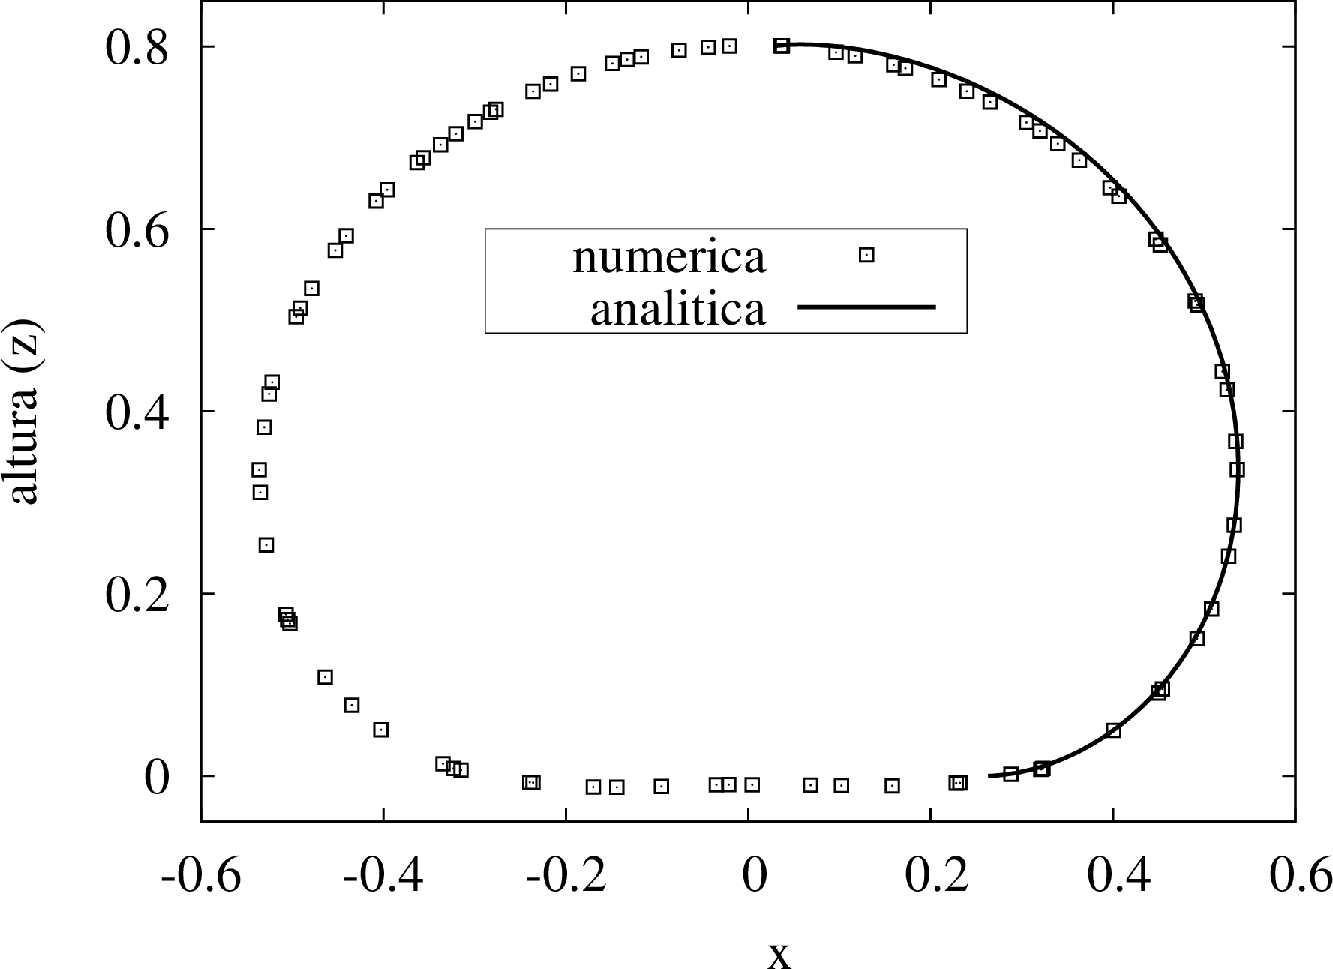
\includegraphics[angle=0, scale=0.5]{figs/sessileShape.pdf}
 	\end{center}
	\caption{Comparação entre a solução numérica do formato da gota
	obtida e a solução
	analítica correspondente para uma gota apoiada com simetria axial.
	A solução analítica é encontrada através da equação de capilaridade
	de Young-Laplace.}
 	\label{fig:sessileShape} 
 \end{figure}

\subsubsection{Ascensão de bolhas confinadas em canais de dimensão
macroscópica e microscópica}

A simulação de escoamentos de bolhas com diâmetro maior que o diâmetro
do canal é um desafio na área de escoamentos multifásicos devido ao seu
grau de dificuldade associado à presença de um filme líquido que separa
bolha e a superfície da parede do canal. Nesta configuração, os efeitos
de pressão e tensão superficial são de extrema importância pois estão
acoplados fortemente e interagem para mudar o campo do velocidades do
escoamento. Além do mais efeitos gravitacionais devem ser considerados
para canais com dimensão da ordem de $10^{-3}$.

A Fig.~(\ref{fig:sucrose}) mostra a progressão temporal de uma bolha do
tipo "Taylor" imersa em uma solução de sacarose. A bolha é iniciada com
o formato apresentado na Fig.~(\ref{fig:sucrose}a) e sua evolução pode
ser acompanhada nas imagens seguintes. Na evolução transiente, a
velocidade da bolha alcança sua máxima velocidade no $t \approx 1$ e sua
velocidade terminal no tempo $t \approx 3.7$, mantendo esta velocidade
durante o restante da simulação. É mostrado que a parte inferior da
bolha oscila durante o estado transiente e converge para a posição final
no tempo $t \approx 7.4$. A Fig.~(\ref{fig:sucroseVel} apresenta a
solução transiente da velocidade do centroide da bolha. Foi observado
uma extrapolação do valor da velocidade entre $t=0$ e $t=1.1$, devido à
deformação inicial da parte inferior da bolha e, consequentemente, a
aceleração de seu centro de massa.

 \begin{figure}[!h]
 	\begin{center}
 		\subfloat[$t=0.00$]
			{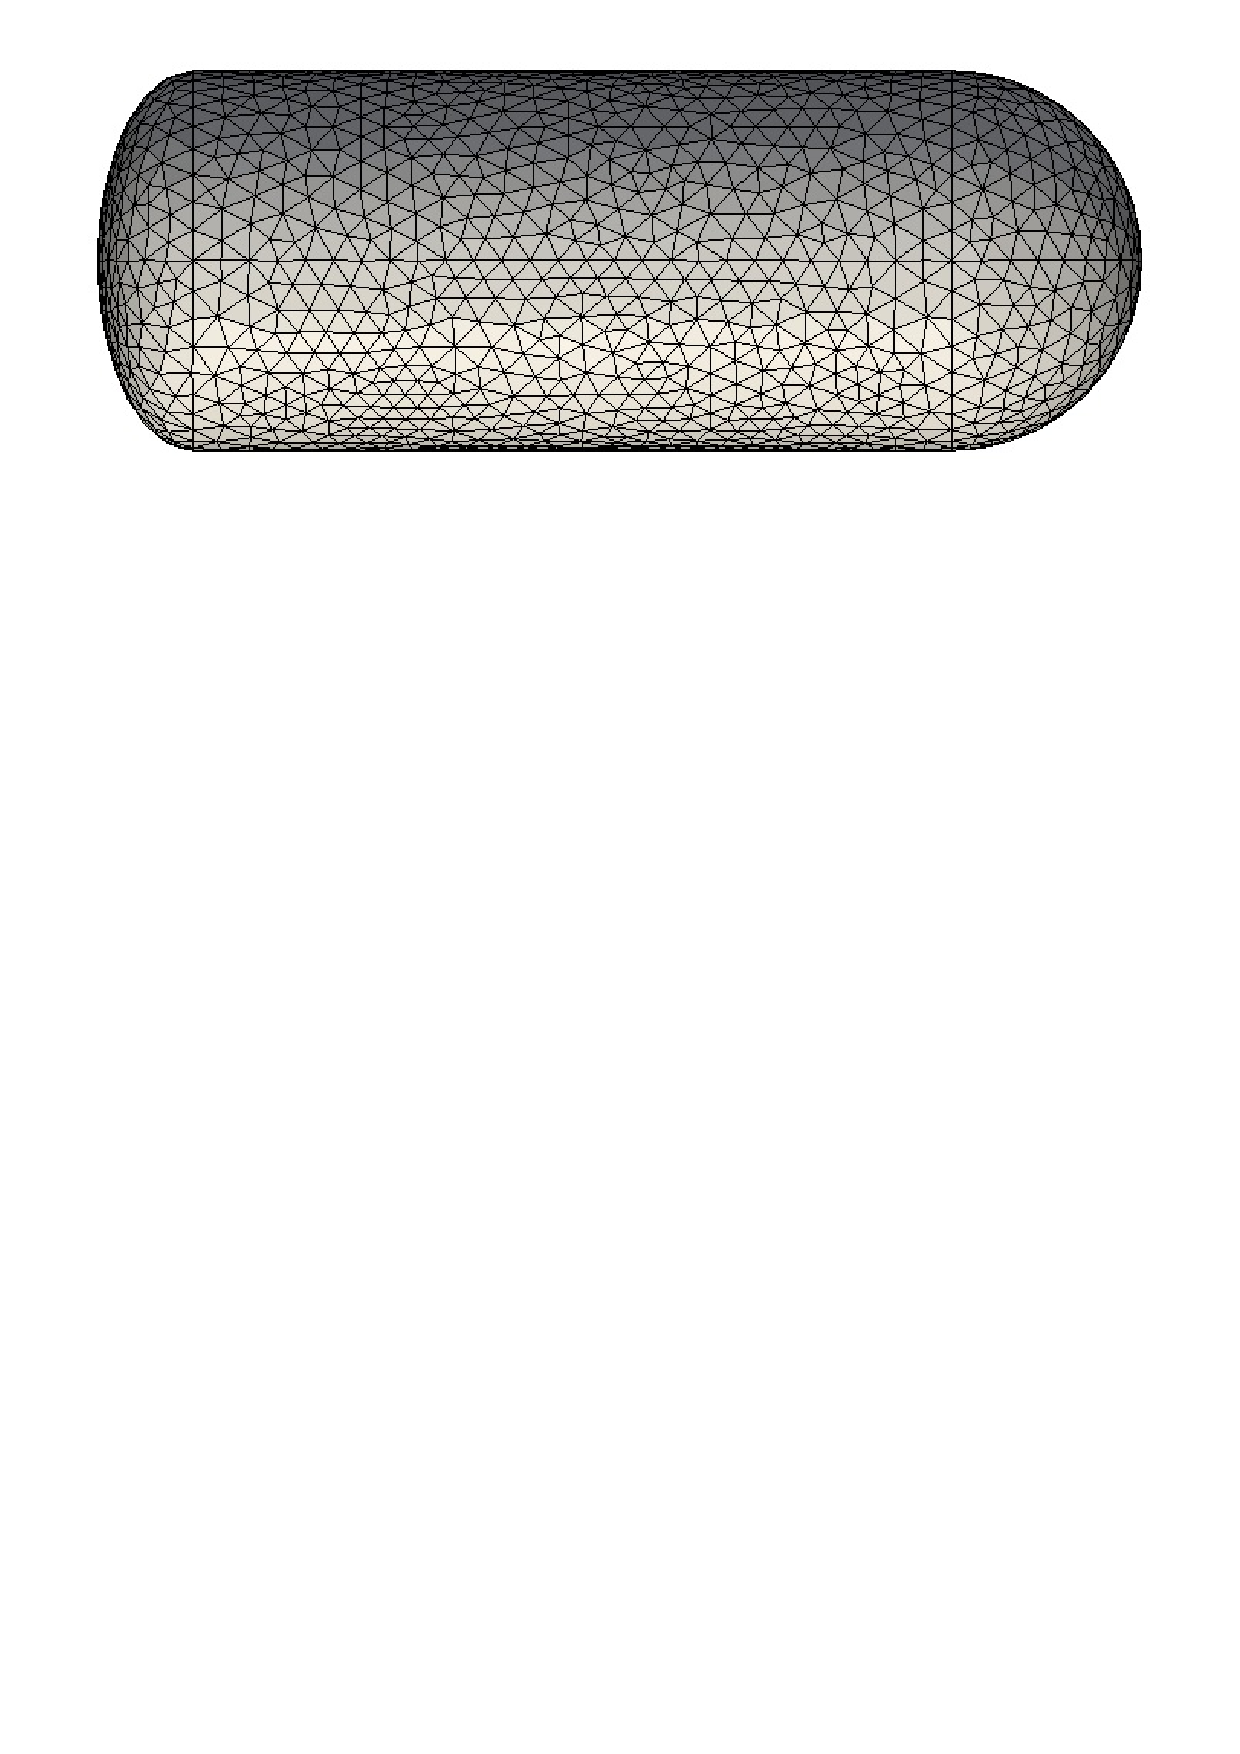
\includegraphics[angle=90,scale=0.3]{figs/sucrose-1.pdf}}
 		\hspace{0.7cm}
 		\subfloat[$t=1.09$]
			{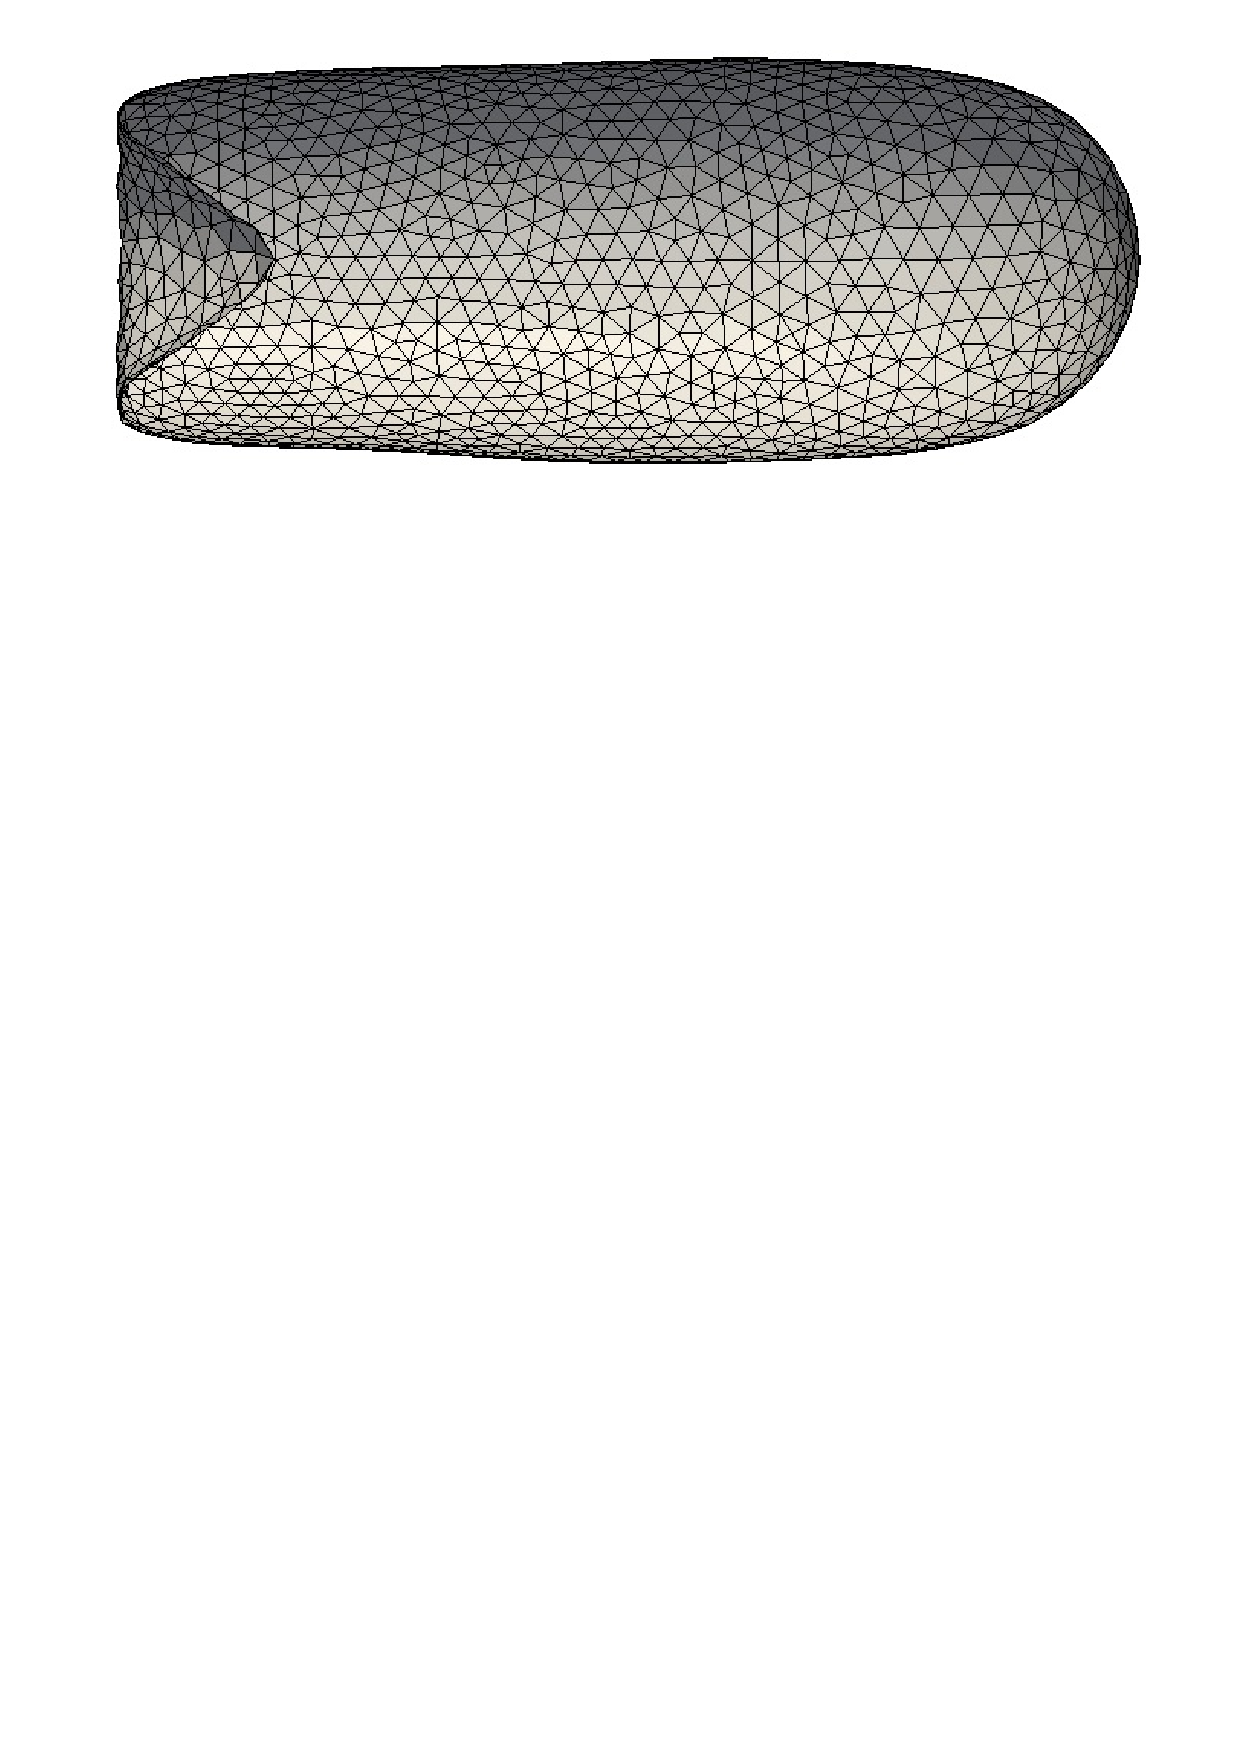
\includegraphics[angle=90,scale=0.29]{figs/sucrose-2.pdf}}
 		\hspace{0.7cm}
 		\subfloat[$t=1.78$]
			{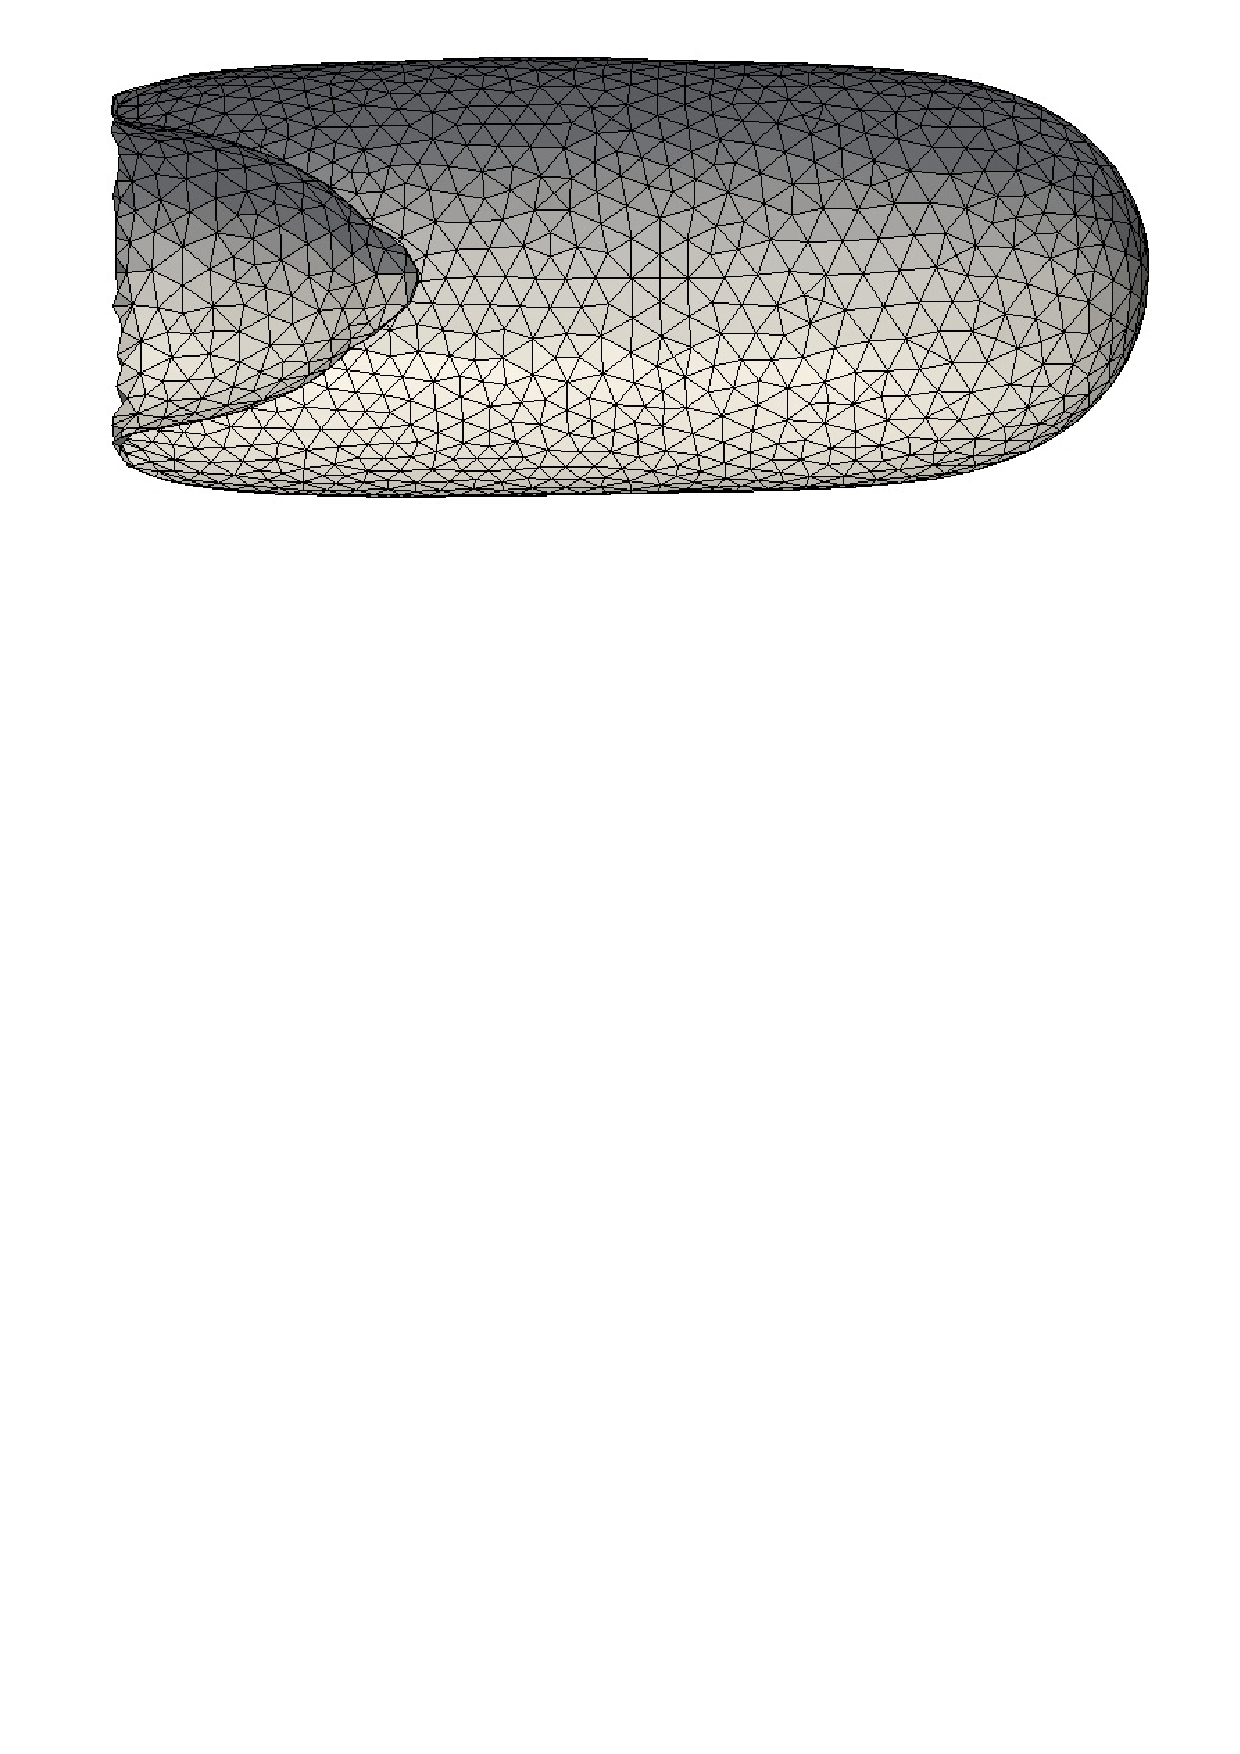
\includegraphics[angle=90,scale=0.29]{figs/sucrose-3.pdf}}
 		\hspace{0.7cm}
 		\subfloat[$t=3.05$]
			{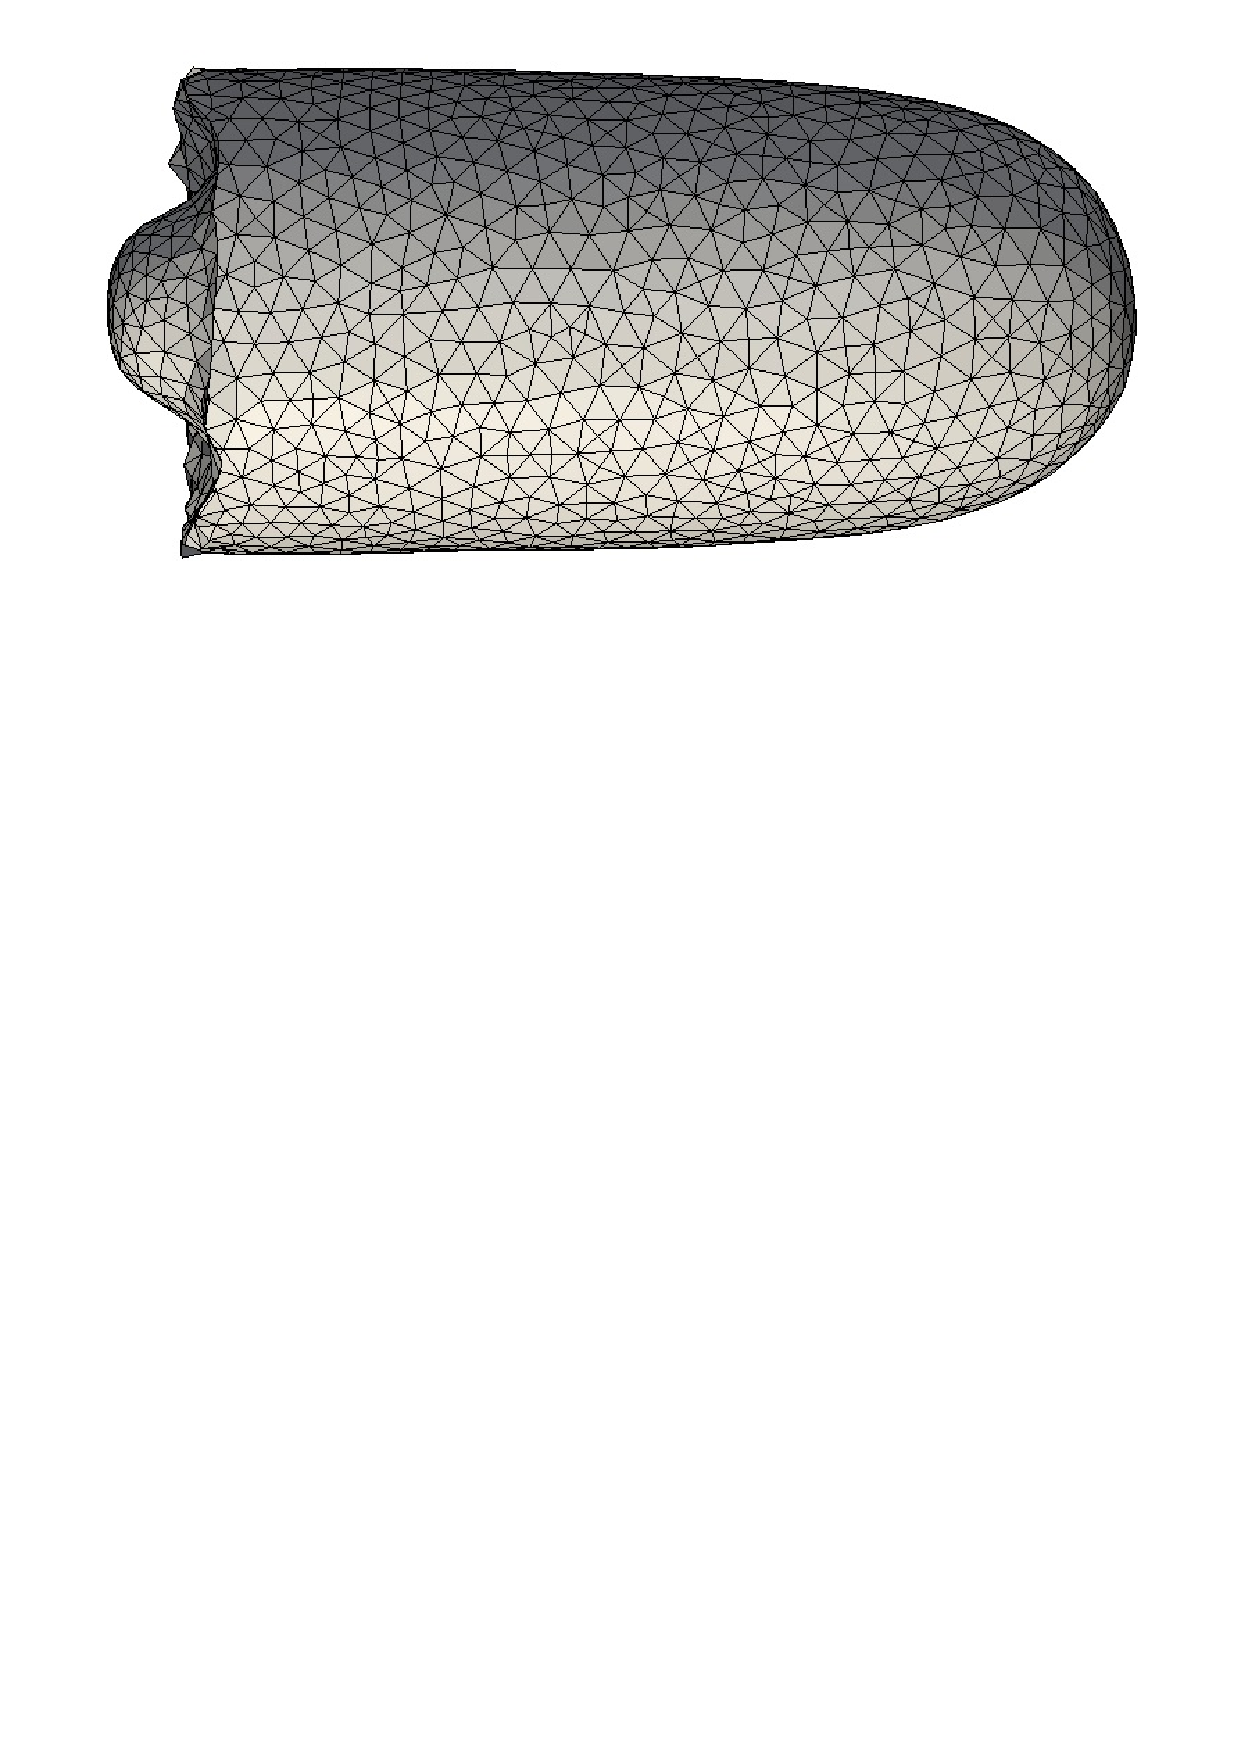
\includegraphics[angle=90,scale=0.29]{figs/sucrose-4.pdf}}
 		\hspace{0.7cm}
 		\subfloat[$t=7.41$]
			{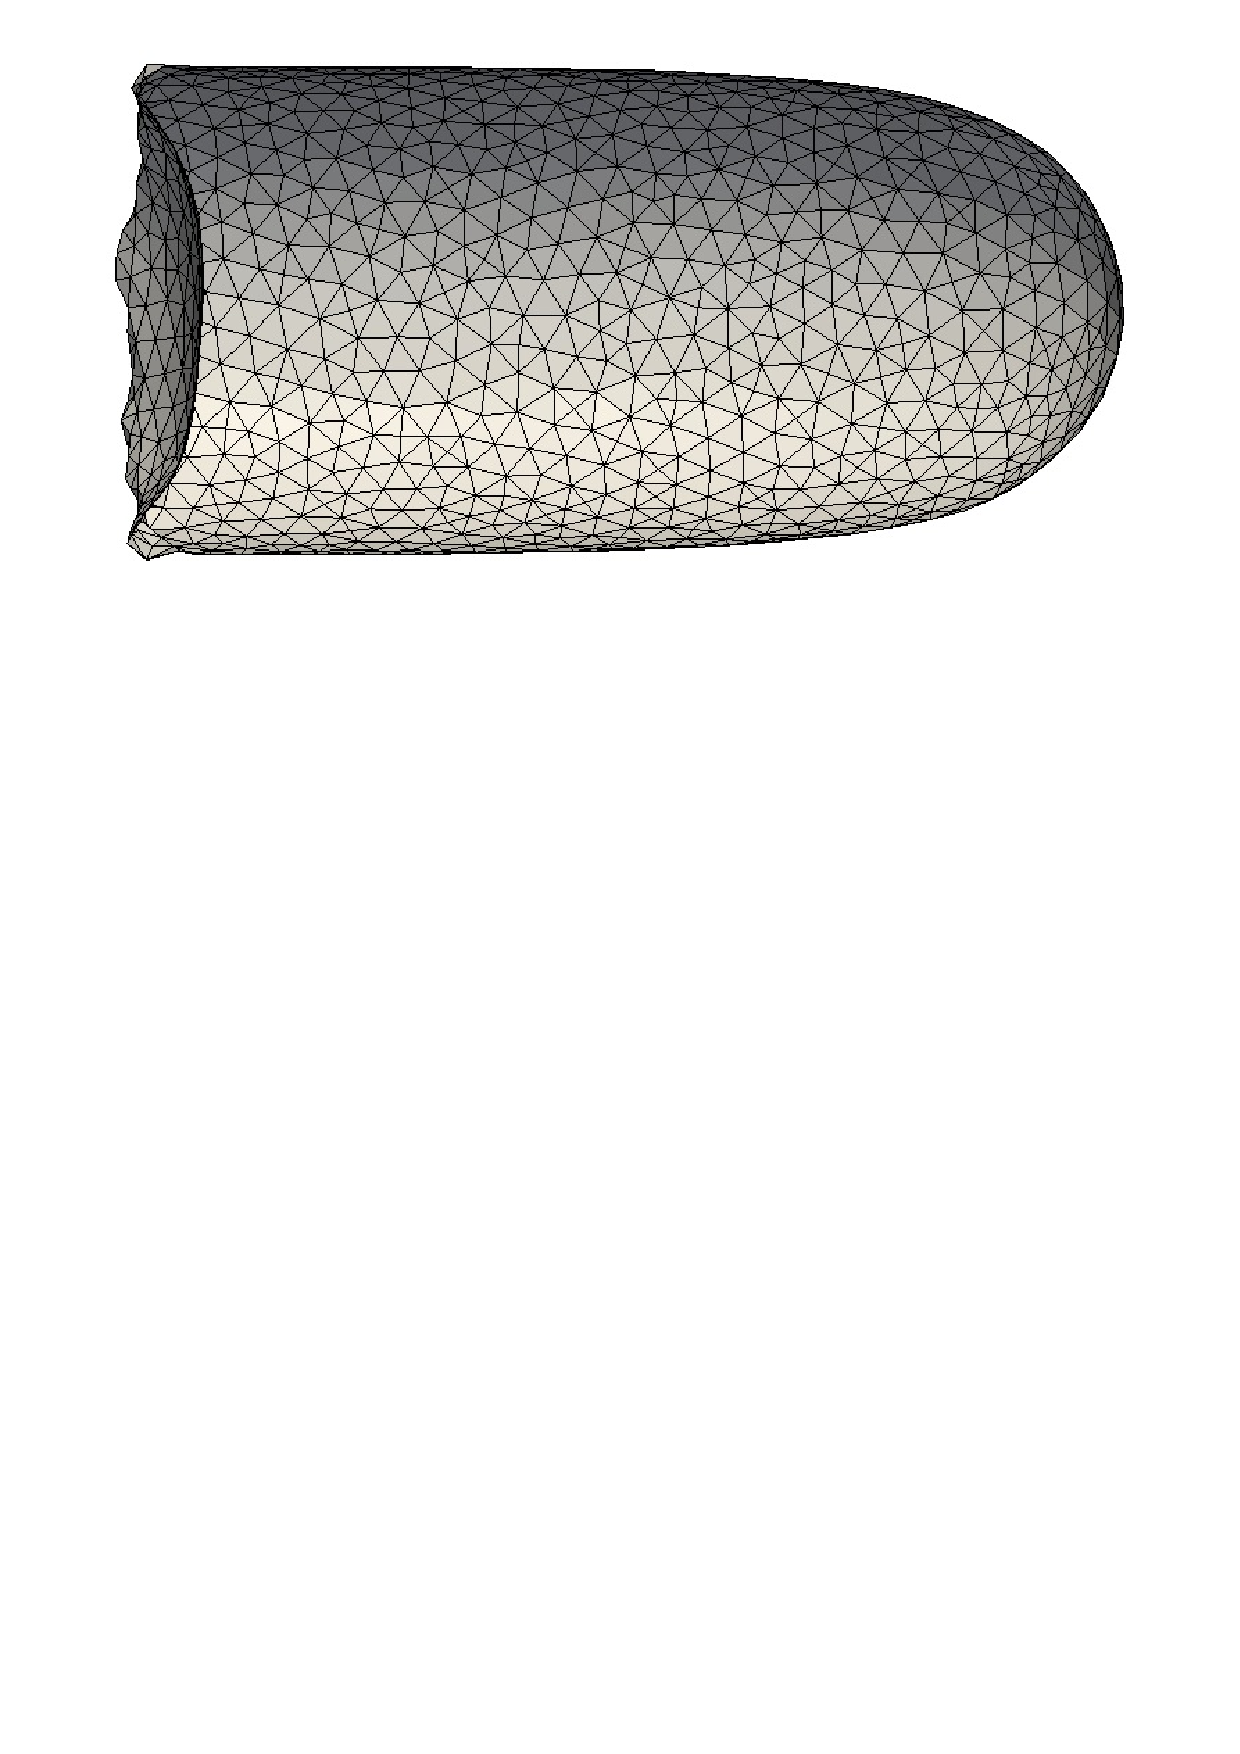
\includegraphics[angle=90,scale=0.29]{figs/sucrose-5.pdf}}
 	\end{center}
	\caption{Evolução da forma da bolha com o tempo para uma bolha de ar
	imersa em uma solução de sacarose. (a) Forma inicial da bolha para
	$t=0$. (b-d) Mudança da forma da bolha para solução transiente no
	tempo. (e) Forma da bolha final com $t=7.41$.} 
	\label{fig:sucrose} 
 \end{figure}


 \begin{figure}[h]
 	\begin{center}
 		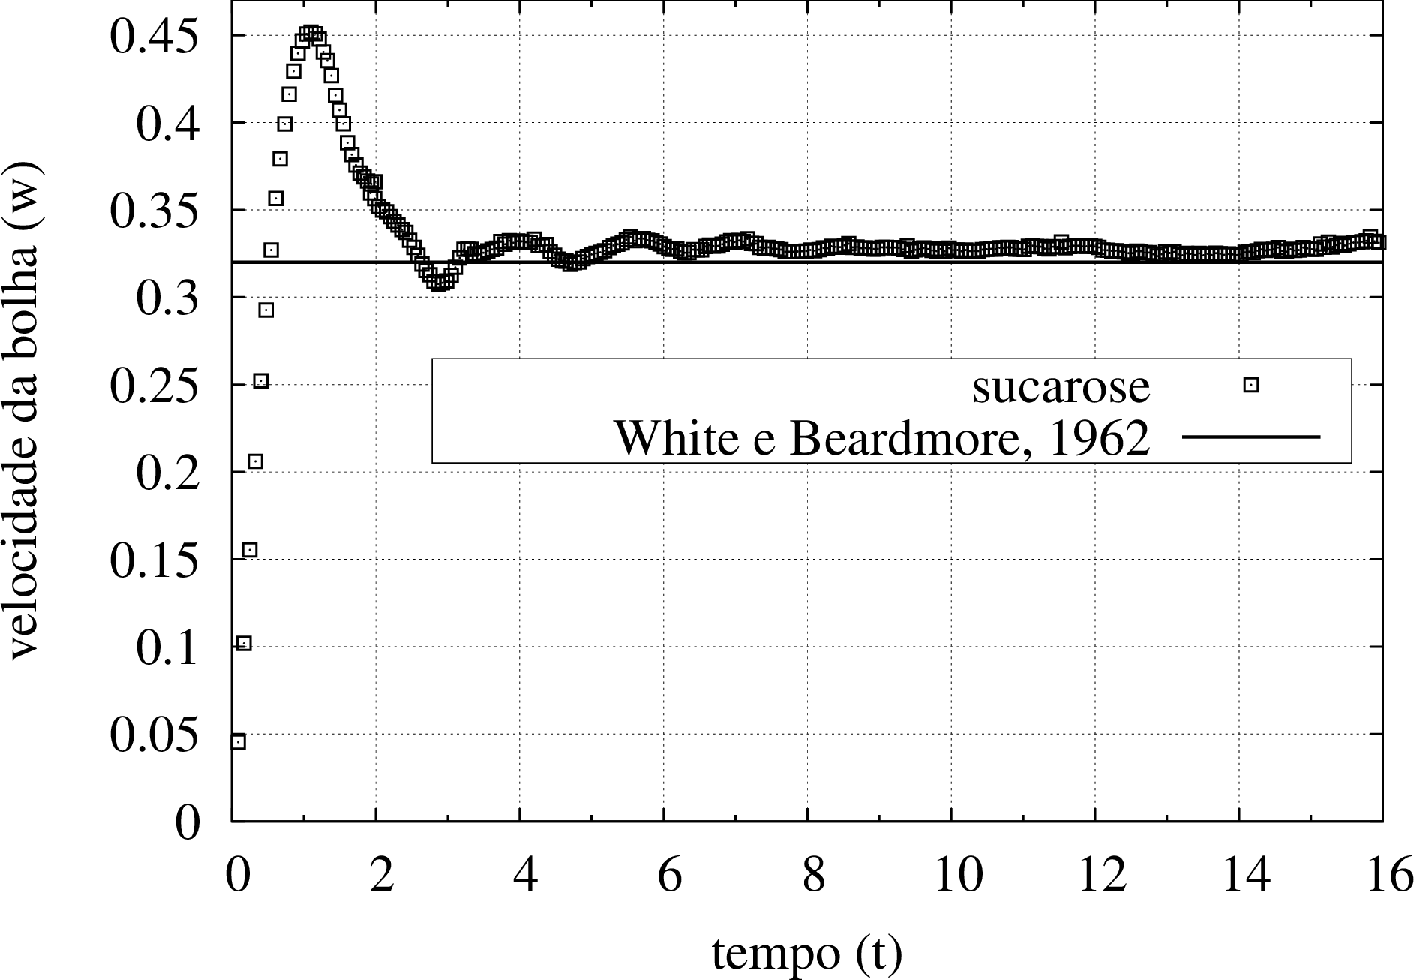
\includegraphics[angle=0, scale=0.5]{figs/sucrose.pdf}
 	\end{center}
	\caption{Elevação de uma bolha de ar do tipo Taylor imersa em uma
	solução de sacarose. A evolução da velocidade de centro de massa da
	bolha é comparada com a velocidade terminal da bolha encontrada no
	mapa de velocidades de \cite{white1962}.}
   \label{fig:sucroseVel}
 \end{figure}

\subsubsection{Escoamento de bolhas em microcanais ondulados}

Nesta seção apresentamos resultados de escoamentos de bolhas em
microcanais ondulados que apresentam variação de diâmetro ao longo de
seu comprimento.  A Fig.~(\ref{fig:sin}) representa a evolução da forma
de uma bolha do tipo Taylor em função do tempo para uma bolha de ar
imersa em uma solução de glicerol em um microcanal ondulado pertinente
ao processo de de produção, estocagem, transporte e consumo de metano da
decomposição de biomassa em reservatórios de hidrelétricas. A forma do
canal é definida por uma função senoidal e a malha numérica utilizada
nesta simulação pode ser observada. Nota-se que a dinâmica do escoamento
faz com que a bolha se deforme quando o diâmetro da tubulação é reduzido
ou aumentado, gerando um efeito de oscilação em sua forma. Para casos
onde a velocidade de escoamento da bolha é elevada, nota-se até mesmo a
ruptura da interface devido à grande oscilação gerada pela redução
seguida de expansão do diâmetro do canal.

 \begin{figure}[!ht]
 	\begin{center}
 		\subfloat[$t=0.00$]
			{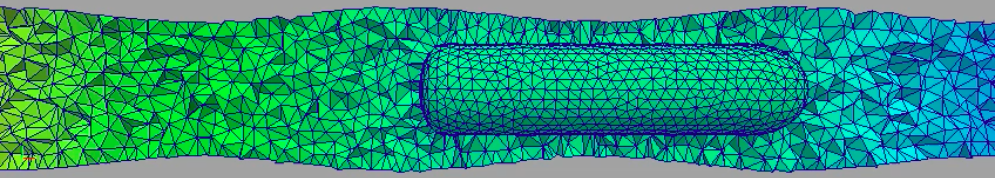
\includegraphics[angle=0,scale=0.305]{figs/sin-0.png}}
 		\hspace{0.7cm}
 		\subfloat[$t=1.09$]
			{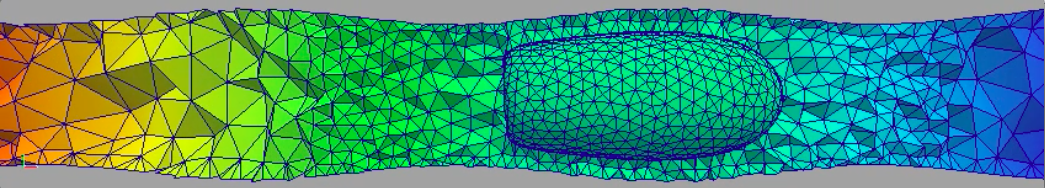
\includegraphics[angle=0,scale=0.29]{figs/sin-1.png}}
 		\hspace{0.7cm}
 		\subfloat[$t=2.15$]
			{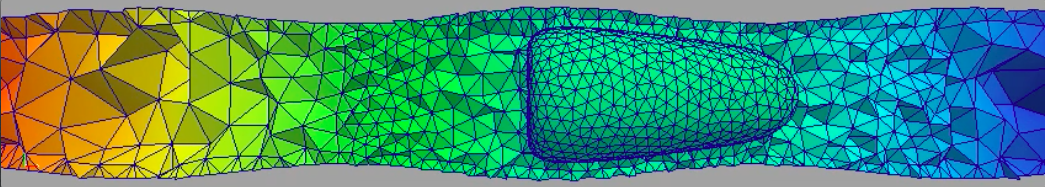
\includegraphics[angle=0,scale=0.29]{figs/sin-2.png}}
 		\hspace{0.7cm}
 		\subfloat[$t=3.71$]
			{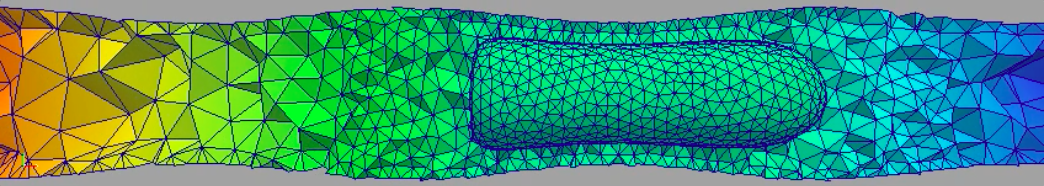
\includegraphics[angle=0,scale=0.29]{figs/sin-3.png}}
 		\hspace{0.7cm}
 		\subfloat[$t=4.05$]
			{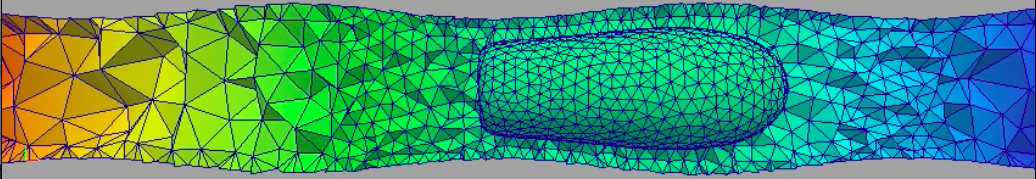
\includegraphics[angle=0,scale=0.29]{figs/sin-4.png}}
 		\hspace{0.7cm}
 		\subfloat[$t=5.18$]
			{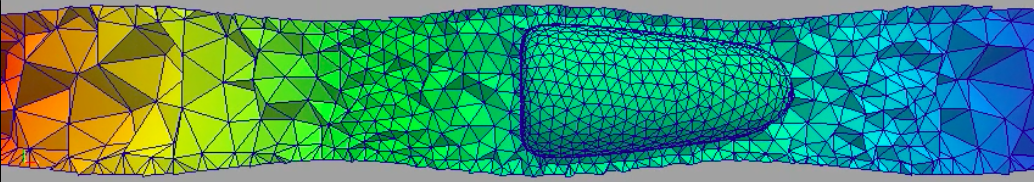
\includegraphics[angle=0,scale=0.29]{figs/sin-5.png}}
 	\end{center}
	\caption{Evolução da forma de uma bolha do tipo Taylor em função do
	tempo para uma bolha de ar imersa em uma solução de glicerol em um
	canal ondulado. A forma do canal é definida por uma função senoidal.
	(a) Forma inicial da bolha para $t=0$. Forma da bolha para solução
	transiente no tempo em (b) $t=1.09$, (c) $t=2.15$, (d) $t=3.71$, (e)
	$t=4.05$, (f) $t=5.18$.} 
	\label{fig:sin} 
 \end{figure}

\subsection{Modelo Axissimétrico}

Uma comparação com modelos tridimensionais e resultados experimentais é
realizada nesta seção para o simulador numérico de modelo com simetria
axial para escoamentos multifásicos envolvendo a composição binária
líquido-gás. Note que a simulação axissimétrica é feita utilizando malha
bidimensional triangular e para sua interpretação física, deve-se
rotacionar o plano de visualização em $360^\circ$.

Na Fig.~(\ref{fig:micro1}), observa-se a evolução de bolha de ar
axissimétrica em ascensão em uma solução de água com açúcar e
viscosidade dinâmica $\mu=2.73$. A bolha é inicialmente ajustada como
esférica (ou um círculo de raio $R=0.5$ em modelo de simetria axial) e,
em seguida, dada a diferença de densidades entre fluidos, a bolha entra
em dinâmica de ascensão, mudando sua forma com a evolução temporal, até
chegar ao estado final de sua forma. Nota-se que a bolha apresenta
formato tampão elipsoidal com formação e desprendimento de vórtices na
parte posterior da bolha.

\begin{figure}[!h]
	\begin{center}
		\subfloat[$t=0.0$]
   		{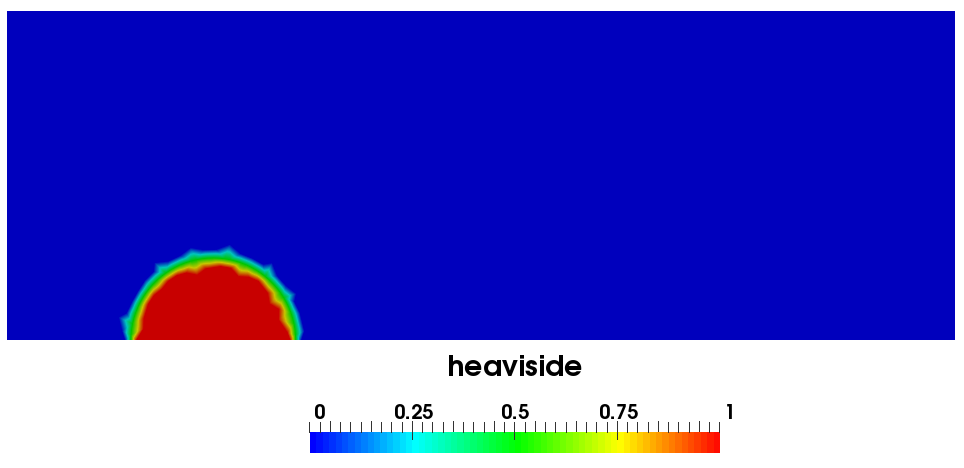
\includegraphics[angle=90,scale=0.25]{figs/rising-00.png}}
		\hspace{0.7cm}
		\subfloat[$t=0.69$]
   		{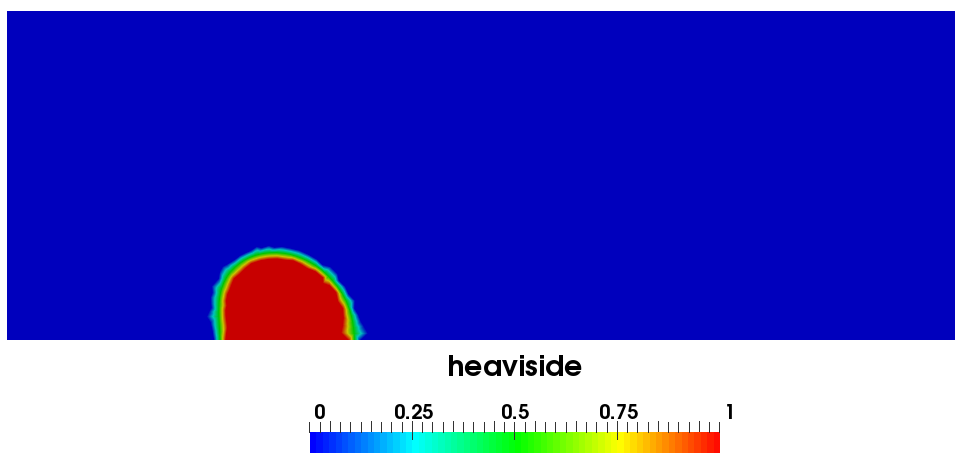
\includegraphics[angle=90,scale=0.25]{figs/rising-01.png}}
		\hspace{0.7cm}
		\subfloat[$t=1.33$]
   		{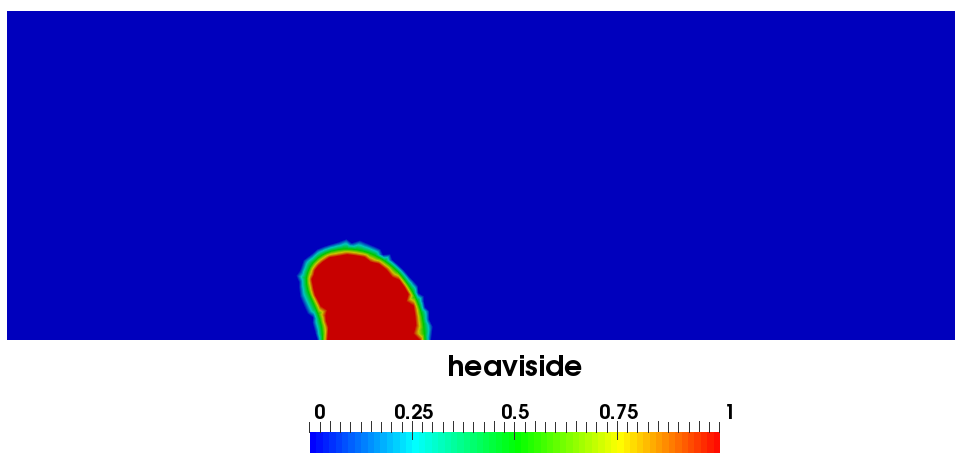
\includegraphics[angle=90,scale=0.25]{figs/rising-02.png}}
		\\
		\subfloat[$t=1.96$]
   		{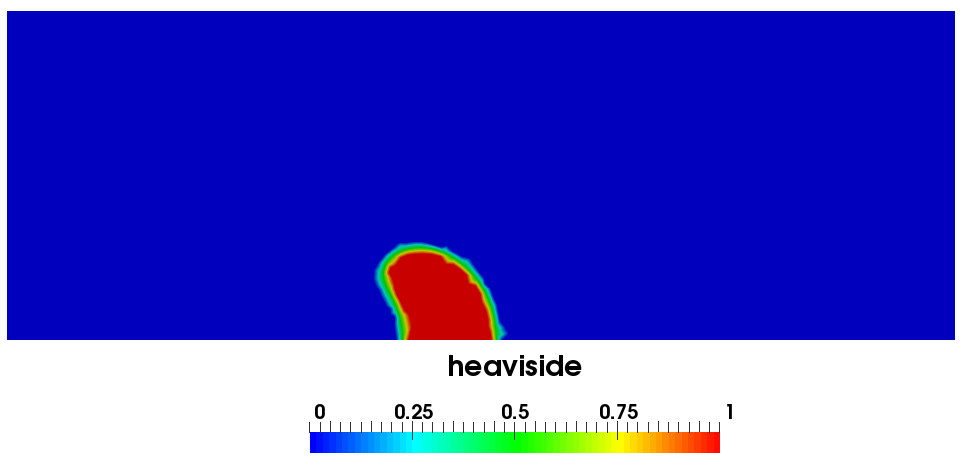
\includegraphics[angle=90,scale=0.25]{figs/rising-03.png}}
		\hspace{0.7cm}
		\subfloat[$t=2.59$]
   		{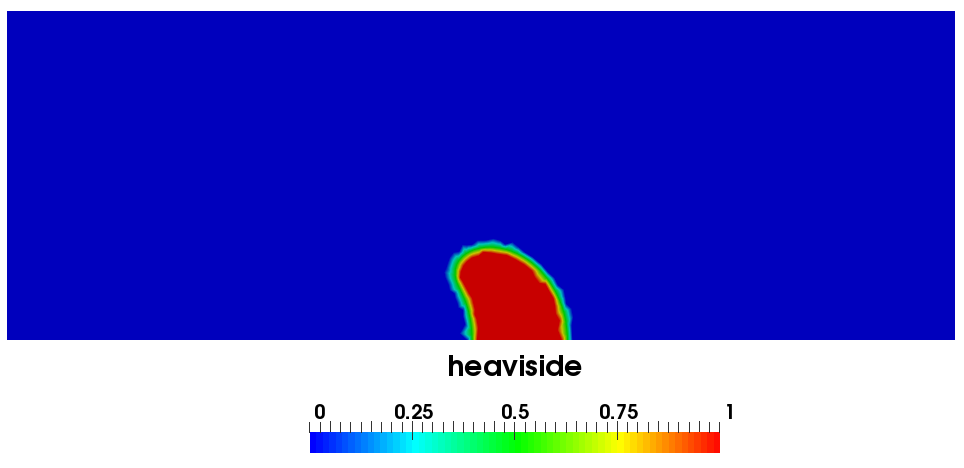
\includegraphics[angle=90,scale=0.25]{figs/rising-04.png}}
		\hspace{0.7cm}
		\subfloat[$t=3.21$]
   		{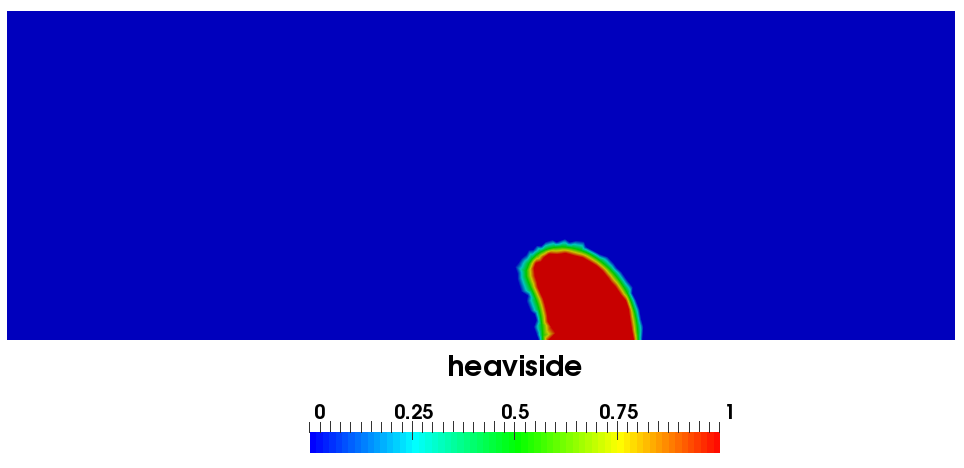
\includegraphics[angle=90,scale=0.25]{figs/rising-05.png}}
	\end{center}
   \caption{Evolução de bolha de ar axissimétrica em ascensão em uma
   solução de água com açúcar e viscosidade dinâmica $\mu=2.73$. (a)
   Bolha inicialmente esférica. (b)-(d) Evolução da forma da bolha e
   (e)-(f) bolha em estado final de forma.} 
   \label{fig:micro1} 
\end{figure}

Uma visualização de campos e malha computacional utilizada nas
simulações é apresentada na Fig.~(\ref{fig:micro2}). A função de
\emph{heaviside} representa um campo de identificação de fases (líquida
e gasosa) e triângulos são utilizados para construção da malha utilizada
nas simulações numéricas. Nota-se que a malha mantem ótima razão de
aspecto, preservando a qualidade do elemento finito e, consequentemente,
diminuindo o erro de discretização numérica.

\begin{figure}[!h]
	\begin{center}
		\subfloat[]
   		{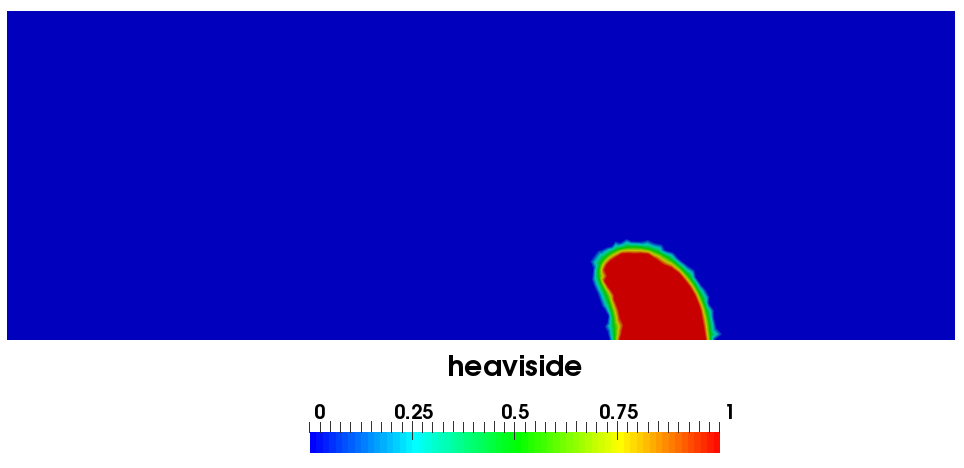
\includegraphics[angle=90,scale=0.25]{figs/rising-06.png}}
   	\hspace{0.7cm}
		\subfloat[]
   		{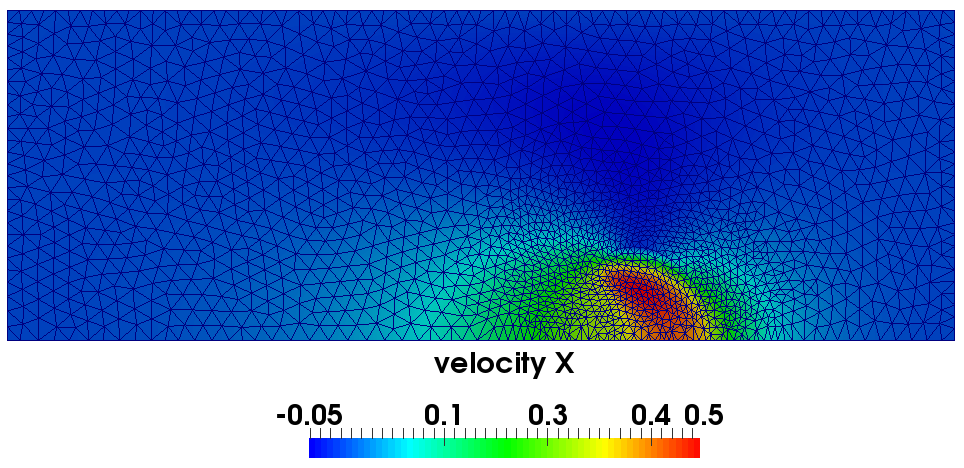
\includegraphics[angle=90,scale=0.25]{figs/rising-07.png}}
	\end{center}
   \caption{Visualização da evolução de bolha de ar axissimétrica para
   o tempo $t=3.85$ (a) campo de identificação de fases (b) malha
   bidimensional de elementos triangulares e campo de velocidade
   vertical.} 
   \label{fig:micro2} 
\end{figure}

Simulação numérica axissimétrica de escoamentos em microcanais com
bolhas confinadas e sua respectiva evolução temporal e espacial é
apresentado na Fig.~(\ref{fig:taylor1}). A bolha de gás (em cor
vermelha) é inicialmente disposta no centro do tubo com diâmetro $D=2R$,
sendo $R$ o raio adimensional da bolha. Por sua vez, a bolha tem
comprimento de $2.5R$, configurando assim um escoamento de bolha tipo
Taylor horizontal. No tempo $t=0.65$ o filme que separa a interface da
bolha (verde) da parede do tupo diminui devido à proporção entre
densidades e viscosidades dos fluidos. Em $t=1.33$ nota-se que o filme
líquido diminuir ainda mais na parte da esquerda do bolha, que configura
o término da bolha, uma vez que a mesma viaja para a direita. No tempo
$t=3.46$ a bolha encontra sua forma final permanente, mantendo-se nesta
forma até o final da simulação para $t>3.46$.

\begin{figure}[!h]
	\begin{center}
		\subfloat[$t=0.0$]
   		{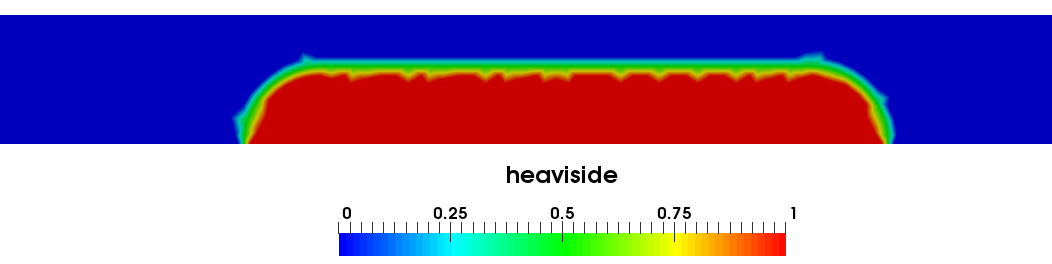
\includegraphics[angle=0,scale=0.2]{figs/taylor-00.png}}
		\hspace{0.7cm}
		\subfloat[$t=0.65$]
   		{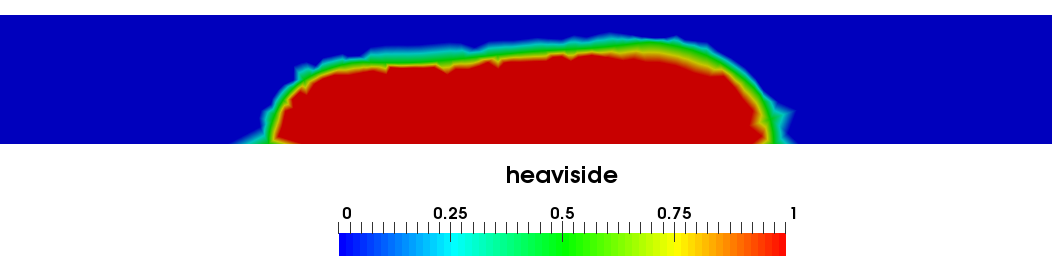
\includegraphics[angle=0,scale=0.2]{figs/taylor-01.png}}
		\\
		\subfloat[$t=1.33$]
   		{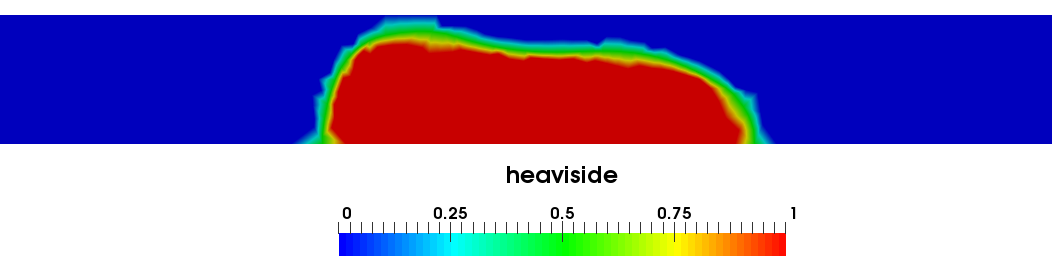
\includegraphics[angle=0,scale=0.2]{figs/taylor-02.png}}
		\hspace{0.7cm}
		\subfloat[$t=2.05$]
   		{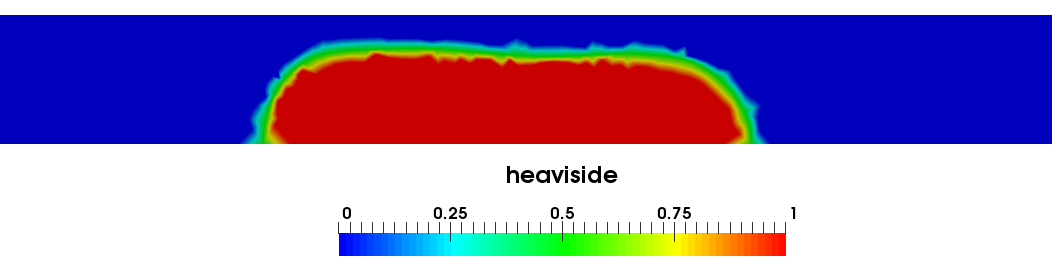
\includegraphics[angle=0,scale=0.2]{figs/taylor-03.png}}
		\\
		\subfloat[$t=2.76$]
   		{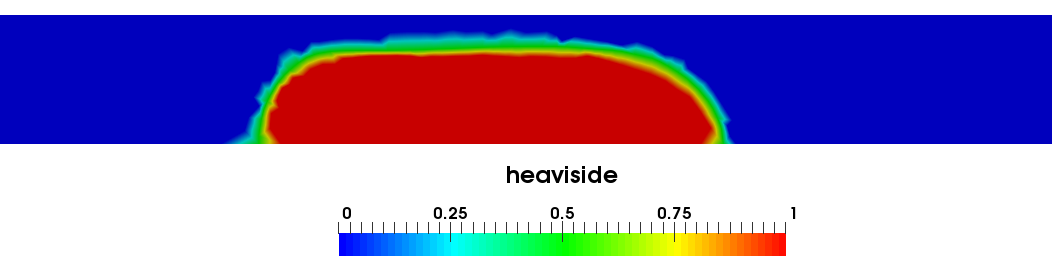
\includegraphics[angle=0,scale=0.2]{figs/taylor-04.png}}
		\hspace{0.7cm}
		\subfloat[$t=3.46$]
   		{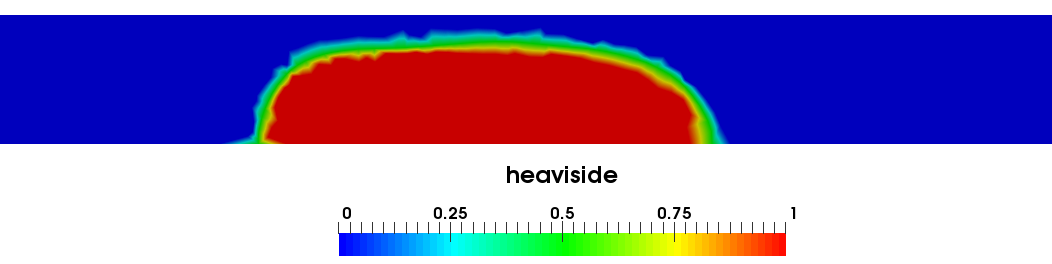
\includegraphics[angle=0,scale=0.2]{figs/taylor-05.png}}
	\end{center}
   \caption{Evolução de bolha do tipo Taylor em microcanais
   axissimétricos com forma contínua. (a) Bolha em forma inicial
   confinada. (b)-(d) Evolução da forma da bolha e (e)-(f) bolha em
   estado final de forma após regime transiente.} 
   \label{fig:taylor1} 
\end{figure}

Na Fig.~(\ref{fig:taylor2}) é apresentada uma visualização para tempo
$t=3.46$ do campo de identificação de fases e da malha bidimensional de
elementos triangulares. Nota-se nesta simulação que a malha mantem
ótima razão de aspecto, preservando a qualidade do elemento finito
e, consequentemente, diminuindo o erro de discretização numérica.

\begin{figure}[!h]
	\begin{center}
		\subfloat[]
   		{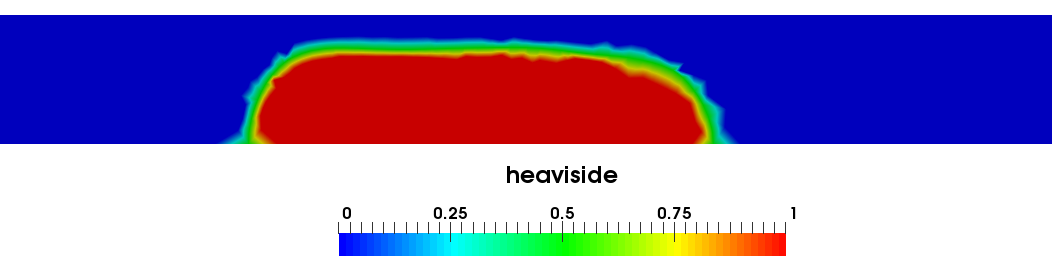
\includegraphics[angle=0,scale=0.2]{figs/taylor-06.png}}
		\hspace{0.7cm}
		\subfloat[]
   		{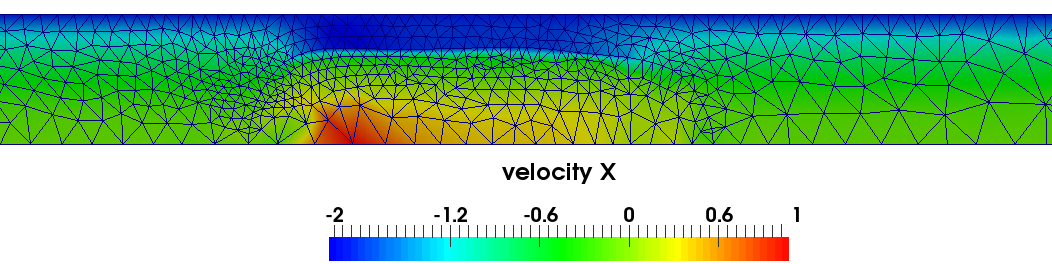
\includegraphics[angle=0,scale=0.205]{figs/taylor-07.png}}
	\end{center}
   \caption{Visualização da evolução de bolha de ar axissimétrica para
   o tempo $t=4.14$ (a) campo de identificação de fases (b) malha
   bidimensional de elementos triangulares e campo de velocidade
   horizontal.} 
   \label{fig:taylor2} 
\end{figure}


\subsection{Modelo de estruturas de não-equilíbrio em sistemas químicos}

Nesta seção de resultados deseja-se mostrar o desenvolvimento do campo
hidrodinâmico acoplado ao perfil de concentrações devido ao movimento de
fluidos em meios porosos. As instabilidade formadas são fortemente
associadas a mudanças de viscosidade e densidade entre diferentes
camadas de um fluido contendo soluto de concentração invariável. Tal
fenômeno ocorrem em grande variedade de aplicações biológicas, químicas
e ambientais, incluindo técnicas de sequestro de $\mathbf{CO_2}$,
hidrologia e aplicações médicas. 

O modelo de estruturas de não-equilíbrio descrito na
Sec.~(\ref{sec:chem}) é testado para diversos perfis de concentração $c$
médios em diversos passos de tempo. A Fig.~(\ref{fig:chem1}) mostra a
evolução dos perfis de concentração calculados pela Lei de Darcy e
aproximação Boussinesq e comparados com sua solução analítica. Na
Fig.~(\ref{fig:chem1}b) a amplitude de diferentes modos de perturbação
de concentração $c$ e da corrente $\psi$ são identificados e
apresentados. No tempo $t=4000$ pode-se observar uma distorção devido ao
aumento da perturbação. No tempo $t=5000$ (ver Fig.~(\ref{fig:chem1}d))
observa-se um perfil de concentração ondulado, com pouca variação de
amplitude na difusão do campo a partir da interface linear. 

 \begin{figure}[h!]
 	\begin{center}
 		\subfloat[]
 			{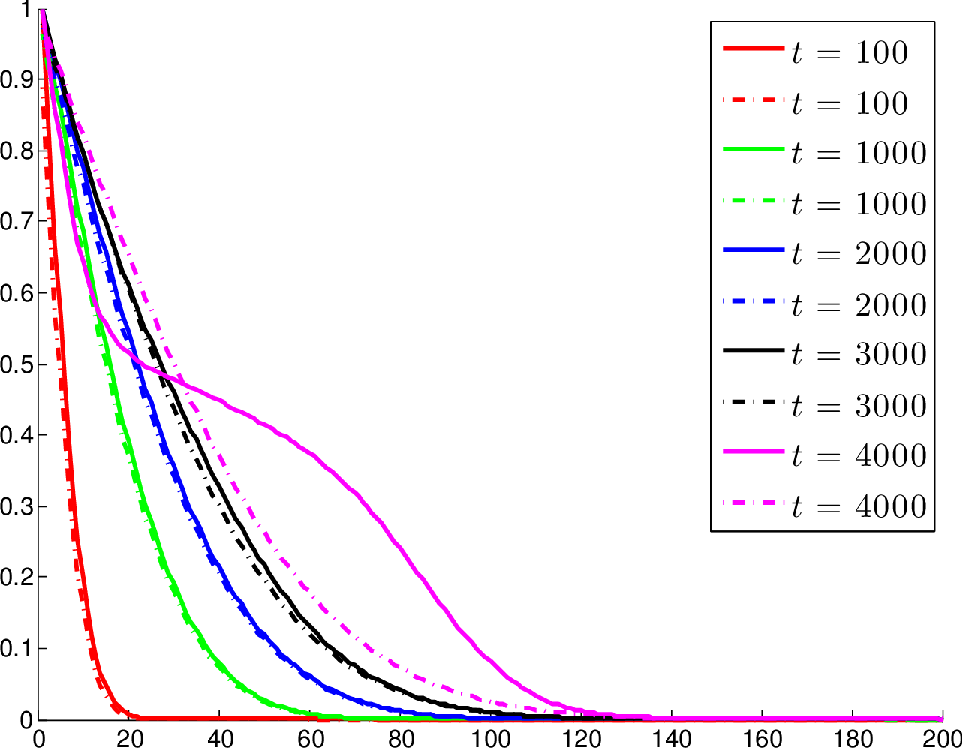
\includegraphics[angle=0, scale=0.4]{figs/5PerfisMedios.pdf}}
 		\hspace{0.7cm}
 		\subfloat[]
 			{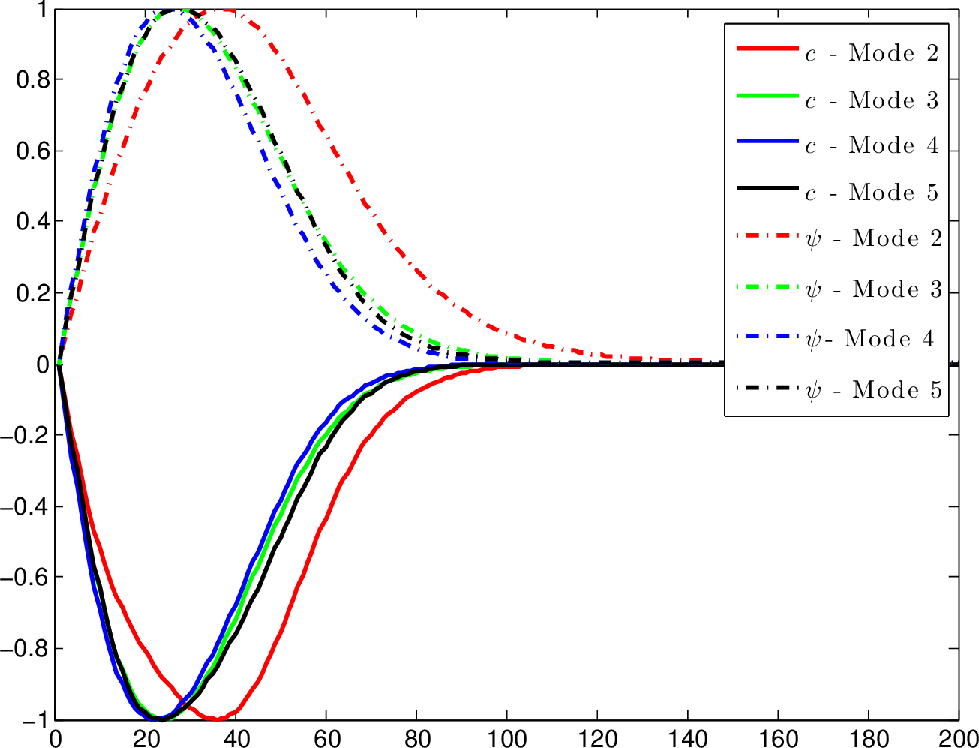
\includegraphics[angle=0, scale=0.4]{figs/psi_e_c_4modos.pdf}}
 	\end{center}
	\caption{(a) Perfis de concentração $c$ médios para diversos passos
	de tempo. As linhas tracejadas representam a solução analítica para
	as soluções numéricas representadas por linhas de mesma cor.(b)
	Amplitude de diferentes modos perturbação de concentração $c$ e da
	função corrente $\psi$.} 
	\label{fig:chem1} 
 \end{figure}

 \begin{figure}[ht!]
 	\begin{center}
 		\subfloat[Modo $n=3$, $t=0$]
			{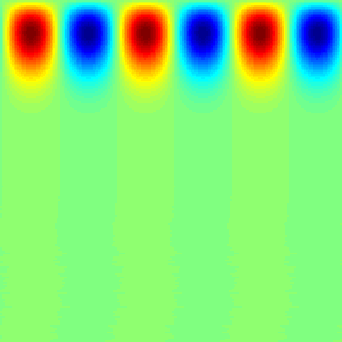
\includegraphics[angle=0,scale=3.0]{figs/chem1.png}}
 		\hspace{0.7cm}
 		\subfloat[$t=3000$]
			{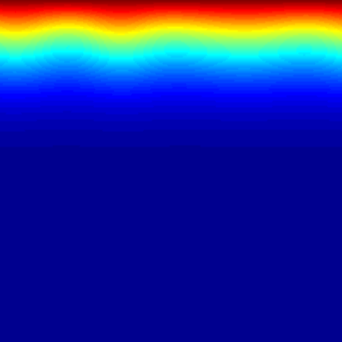
\includegraphics[angle=0,scale=3.0]{figs/chem2.png}}
 		\\
 		\subfloat[$t=4000$]
			{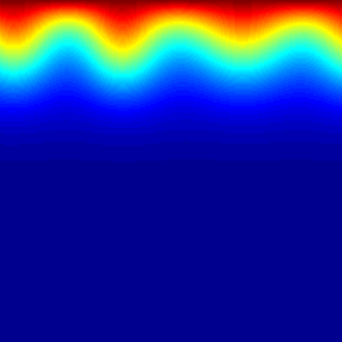
\includegraphics[angle=0,scale=3.0]{figs/chem3.png}}
 		\hspace{0.7cm}
 		\subfloat[$t=5000$]
			{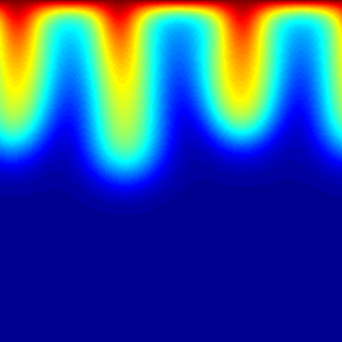
\includegraphics[angle=0,scale=3.0]{figs/chem4.png}}
 	\end{center}
	\caption{(a) Visualização da função corrente $\psi$ para a simulação
	numérica proposta para este projeto. (b)-(d) Evolução temporal e
	espacial do perfil de concentração para o modo $n=3$ em diversos
	tempos de simulação.} 
	\label{fig:chem2} 
 \end{figure}

Na Fig.~(\ref{fig:chem3}), uma comparação de perfis de concentração para
interface plana e interface curva é feita. É possível notar que a
deformação da interface através de uma perturbação senoidal (ondulada)
(ver Fig.~(\ref{fig:chem3}b) provoca intensa instabilidade no campo de
concentração, com padrão de perfil de concentração diferente se
comparado ao modelo de interface linear. Os resultados aqui apresentados
para o modelo de estruturas de não-equilíbrio em sistemas químicos
apresenta concordância com experimentos realizados por grupo de pesquisa
parceiros deste projeto de pesquisa.

 \begin{figure}[h]
 	\begin{center}
 		\subfloat[]
			{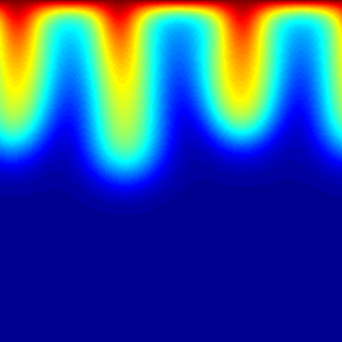
\includegraphics[angle=0,scale=3.0]{figs/chem4.png}}
 		\hspace{0.7cm}
 		\subfloat[]
			{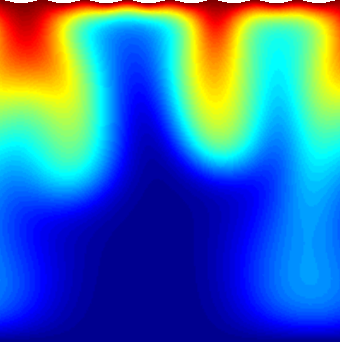
\includegraphics[angle=0,scale=3.0]{figs/chem4-forced.png}}
 	\end{center}
	\caption{Comparação dos perfis de concentração para (a) interface plana
	e (b) interface curva. Note que a deformação da interface provoca
	intensa instabilidade no campo de concentração.} 
	\label{fig:chem3} 
 \end{figure}

\clearpage

\section{Produção Científica}

Abaixo estão listados os artigos publicados em canais de comunicação
internacional em que o pesquisador bolsista teve participação intensiva.

\begin{itemize}
	\item Finite Element Simulation of Fingering in Convective Dissolution in
		  Porous Media Rachel M. Lucena, Norberto Mangiavacchi, José
		  Pontes, Anne De Wit, Gustavo Anjos, JCIS,
		  doi:10.6062/jcis.2015.06.01.0091 -- 2015, \textbf{aceito para
		  publicação}.
	\item Comparative CFD Simulations of Gas Transport in Slug Flow from
		  Periodic Arrays with Single or Multiple Bubbles G. P.
		  Oliveira, N. Mangiavacchi, G. Anjos, J. Pontes, J. R. Thome,
		  JCIS, doi: 10.6062/jcis.2014.05.02.0086 -- 2015,
		  \textbf{aceito para publicação}.
	\item ALE-FEM for two-phase flows with heat and mass transfer in
	      microchannels, G.R. Anjos, N. Mangiavacchi, J. Pontes, J.R. Thome,
		  interPACK -- 2015
	\item Finite Element Simulation of Fingering in Convective Dissolution in
	      Porous Media Rachel M. Lucena, Norberto Mangiavacchi, José Pontes,
	      Anne De Wit, Gustavo Anjos, CCIS -- 2014
	\item Comparative CFD Simulations of Gas Transport in Slug Flow from
		  Periodic Arrays with Single or Multiple Bubbles G. P.
		  Oliveira, N. Mangiavacchi, G. Anjos, J. Pontes, J. R. Thome,
		  CCIS -- 2014.
	\item Topological Remeshing and Locally Supported Smoothing for
	      Bubble Coalescence in Two-Phase Flows
		  Gustavo Charles P. de Oliveira, Norberto Mangiavacchi, Gustavo Anjos
		  John R. Thome, COBEM -- 2013
	\item Finite Element Analysis of Pressure-Driven Laminar Flow Inside
	      Periodically Staggered Arrays
		  Gustavo Charles P. de Oliveira, Gustavo R. Anjos, José Pontes,
		  Norberto Mangiavacchi, CONEM -- 2014
	\item 3D Moving Mesh Finite Element Method for Two-Phase Flows, G.R
	      Anjos, N. Borhani, N.  Mangiavacchi, J.R. Thome,  Journal of
		  Computational Physics, doi:10.1016/j.jcp.2014.03.067 -- 2014
	\item Numerical Simulation of a Periodic Array of bubbles in a
		  channel N. Mangiavacchi, G.C.P. Oliveira, G. Anjos and J. R.
		  Thome, PAMAC -- 2013
	\item A Survey of Results Concerning Steady Solutions and the
	      Stability of a Class of Rotating Flows
		  José Pontes, Norberto Mangiavacchi, Gustavo Rabello dos Anjos,
		  Carlos Mendeza, Rachel Manhães de Lucena, Gustavo C. P.
		  Oliveira and Davi V. A. Ferreira, CCIS -- 2014
\end{itemize}

\section{Plano de Trabalho}

O plano de trabalho proposto para o período total de 19 meses (10
bimestres) de projeto pode ser encontrado na Fig.(\ref{fig:plano}) ,
juntamente com a etapa final do projeto. Nota-se o pesquisador bolsista
foi aprovado no concurso público para professor adjunto do Departamento
de Engenharia Mecânica da Universidade do Rio de Janeiro, tomando posse
no dia 14 de julho de 2014. Em decorrência deste fato, o projeto teve
seu prazo reduzido para final de julho de 2015, totalizando 19 meses (10
bimestres). 

 \begin{figure}[hb!]
 	\begin{center}
 		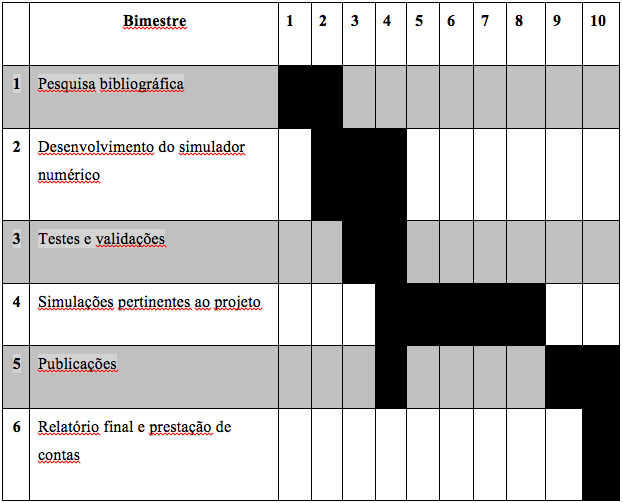
\includegraphics[angle=0, scale=0.75]{figs/plano.png}
 	\end{center}
 	\caption{Plano de trabalho proposto para o período inicial de
	execução do projeto Bolsa de Atração de Jovens Talentos - CAPES.}
 	\label{fig:plano} 
 \end{figure}


\section{Conclusão}

A pesquisa bibliográfica foi realizada com sucesso, onde o bolsista
identificou os pontos mais importantes da modelagem matemática e
implementação numérica para realização de sua pesquisa. A partir do 2o.
bimestre foi iniciado o desenvolvimento do simulador numérico, onde
novas funcionalidades foram incorporadas ao já existente código. Dentre
estes, as seguintes etapas foram realizadas com sucesso:

\begin{itemize}
	\item testes de escoamentos multifásicos com ondas capilares em
	      bolhas;
	\item estudo e desenvolvimento de modelo em três dimensões e axissimétrico
	      para escoamentos multifásicos;
	\item realização de experimentos computacionais de
		  decomposição de biomassa e produção de gases com sedimentação
		  de material orgânico; de medição da sedimentação/ressuspensão
		  e consumo de produtos;
	\item validação dos modelos desenvolvidos para sistemas existentes com
	      utilização de tecnologia de última geração;
	\item estudo e desenvolvimento de modelos tridimensionais e axissimétricos
		  para simulação numérica de estrutura de não-equilíbrio em
		  sistemas químicos, biológico e ambientais;
\end{itemize}

Foi incorporada ao simulador numérico como módulo computacional a
paralelização da solução do sistema linear para cálculo intensivo em
\textit{clusters}, através do desenvolvimento de novos
precondicionadores para a aceleração dos métodos iterativos implantados
e métodos mais eficientes de cálculo de tensão superficial. 

É importante notar que o pesquisador bolsista desenvolveu, além de seu
plano de trabalho inicial, um simulador de escoamentos bidimensional em
linguagem de \textit{script} PYTHON para uso acadêmico, que servirá de
apoio nas aulas ministradas por ele em cursos de graduação e
pós-graduação.

Diversos testes e validações foram realizados com sucesso e os
resultados podem ser encontrados na seção de Resultados Obtidos, bem
como algumas simulações pertinentes ao projeto. O pesquisador bolsista
participou ativamente das publicações relacionadas na seção Produção
Científica usando as funcionalidades incorporadas ao simulador através
deste projeto. 

Os artigos científicos foram publicados em canais de
comunicação internacional de excelência na área de conhecimento CAPES -
Engenharia 3, durante a duração do projeto. Finalmente, a prestação de
contas e a entrega do relatório final foram devidamente alocadas no
final do período proposto deste projeto.  
	
\section{Referências Bibliográficas}
\bibliographystyle{plain}
\bibliography{$HOME/projects/misc/latex/referencias}

\end{document}	

\typeout{ ****************** End of file main.tex ****************** }

